\documentclass[12pt,notitlepage,a4paper]{report}
\usepackage[
    font=avenirnext,
    pdfkeywords={User Guide, cronologic, ADC, time-to-digital converter,
                 Ndigo5G-10},
]{cronologicug}

%%% set fonts and colors according to CI styleguide
\definecolor{lbcolor}{gray}{0.9} % background of code listings

\newcommand{\ugrev}{1.3.1} % also update in NdigoUGRev.tex

\title{Ndigo5G-10 -- User Guide, Rev. \ugrev}
\author{cronologic GmbH & Co. KG}

\definecolor{org}{RGB}{237,120,0}
\definecolor{gry}{RGB}{ 157,157,156}
\definecolor{crongrey}{gray}{0.5} %Variablendeklaration API
\definecolor{cronorange}{RGB}{237, 120, 0}
\definecolor{cronblue}{RGB}{55, 110, 181}
\definecolor{cronblack}{RGB}{0,0,0}
\newcommand{\codeexamplesize}{\footnotesize}

\begin{document}
    \RaggedRight
    \thispagestyle{empty}
\begin{tikzpicture}
\draw[inner sep=0pt] node at (0,0)   { 
\includegraphics[width=\textwidth]{figures/cronologic.pdf}};
\end{tikzpicture}

\begin{minipage}{0.83\textwidth}
\begin{tabular}{l}


\begin{tikzpicture}
\draw[inner sep=0pt] node at (-8.3,1){\fontsize{20}{2}\selectfont
\cronoheaderfont 
{\textcolor{org}{Ndigo5G-PCIe}}};

\draw[align=center] node at (-8.3,0){\fontsize{20}{2}\selectfont
\sffamily \textcolor{org}{USER GUIDE}};
\end{tikzpicture}
\\ \vspace{5pt}
%{\efbox{
%\hspace{-10pt}
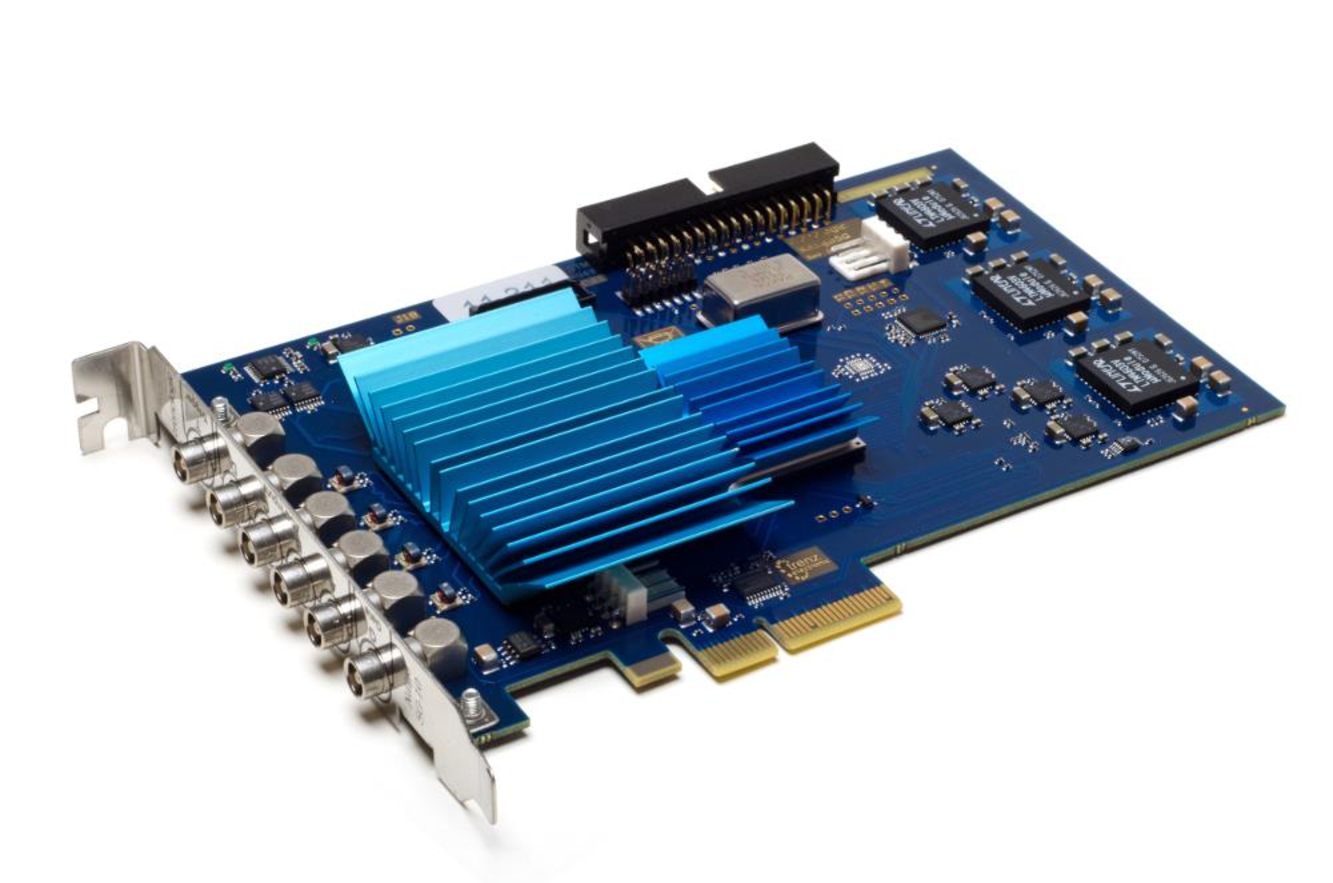
\includegraphics[width=120mm,height=150mm,keepaspectratio]{figures/Title5G.pdf}
%}}
\\
\end{tabular}
\end{minipage}
\begin{minipage}{0\textwidth}
\vspace{25pt}

\begin{tikzpicture}
\draw[inner sep=0pt] node at (0,-5){ 
\fontsize{100}{2}\selectfont
\bfseries \textcolor{org}{ \rotatebox{90}{Ndigo5G-PCIe}}};
\end{tikzpicture}
\end{minipage}

\vspace{-25pt}
\begin{minipage}{0\textwidth}

\begin{tikzpicture}
\draw[inner sep=0pt] node at (-3,-18){\fontsize{20}{2}\selectfont
\sffamily \textcolor{gry}{~\url{www.cronologic.de}}};
\end{tikzpicture}
\end{minipage}
\newpage

    \cleardoublepage
    % \newpage
    \tableofcontents
    \clearpage
    \chapter{Introduction}
        % SVN Info:
% $Date: 2019-06-04 12:35:07 +0200 (Di, 04 Jun 2019) $
% $Rev: 4976 $
% $Author: andreas $
The Ndigo5G is a digitizer and transient recorder designed to sample relatively shorts pulses in rapid repetition. It produces a stream of output packets, each containing data from a single trigger event together with a timestamp.
\section{Features}
    \begin{itemize}
        \item 10 bit dynamic range
        \item Up to 5\,Gsps sample rate (in 1-channel mode)
        \item Up to four ADC channels with configurable DC offsets
        \item Two digital control inputs for gating and triggering, one of
              which can be used as a TDC
        \item Advanced zero suppression to massively reduce data load
        \item PCIe 1.1 x4 interface with 800\,MB/s throughput
        \item Possibility to synchronize up to eight boards
        \item Extension board with four additional digital inputs
        \item Onboard 10\,MHz oscillator with a stability of 25\,ppb, or
              possibility to use external 10\,MHz clock
    \end{itemize}
    \chapter{Hardware}
        % SVN Info:
% $Date: 2021-04-16 11:36:40 +0200 (Fr, 16 Apr 2021) $
% $Rev: 5271 $
% $Author: andreas $
\section{Installing the Board}
	%
	\balance
	%
The Ndigo5G board can be installed in any x4 (or higher amount of lanes) PCIe slot. If the slot electrically supports less than 4 lanes, the board will operate at lowerdata throughput rates.\par
Please ensure proper cooling of the device. The Ndigo5G has an onboard temperature detection. If the ADC chip temperature exceeds 90$^{\circ}$C a warning is issued to the device driver. In case the temperature is higher than 95$^{\circ}$C the ADC is disabled to avoid damage. Using a PCI-slot cooler is in many cases an appropriate solution to circumvent problems caused by overheating if the board is used inside a PC. The Ndigo-Crate will provide sufficient cooling under normal operating conditions.\par
  
Using a single Ndigo5G, no further connections need to be made. For applications that require more than 4 ADC channels, several Ndigo boards can be operated in sync. Any board of the Ndigo product line can be synced to other Ndigo boards, allowing, for instance, for a combination of high speed ADCs (Ndigo5G) and slower high resolution ADCs (Ndigo250M-14) or the upcoming Ndigo TDC.\par
The signals used for board synchronization and inter-board triggering are transferred on a bus be-tween the boards. Join all C2 connectors (see Figure \ref{fig:schematics} on page \pageref{fig:schematics}) on the boards using a ribbon cable. Both ends of the bus need to be terminated properly. If using a Ndigo Crate, connectors providing the termination are located on the crate mainboard next to the PCIe slots to the extreme left and right. For more details, please refer to the Ndigo Crate user guide. In applications that use only a few Ndigo boards installed directly inside a PC, termination PCBs available from cronologic can be used.\par
Ndigo5G's standard device driver can be used to read out all boards and acquire data. For more complex scenarios, using the cronoSync-library, which is part of cronoTools, is recommended. The cronoSync library is provided with the Ndigo device driver. Please refer to the cronoTools user guide for more information.
%
\begin{figure*}[ht]
		\begin{center}
			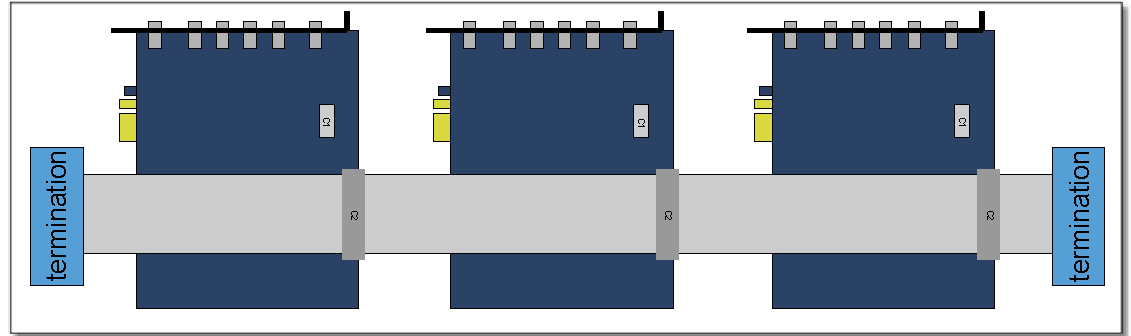
\includegraphics[width=\textwidth]{figures/Ndigo_Intercon.pdf}
		\caption{If several Ndigo boards are connected to work in sync , the boards must be 
connected using a ribbon cable as bus for synchronization and trigger signals. At both 
ends of the cable, proper termination is required.}
		\end{center}
	\end{figure*}
	%
\section{Ndigo5G External Inputs and Connectors}
	\subsection{Connectors}
	%
		The inputs of the Ndigo5G are located on the PCI bracket. Figure \ref{fig:schematics} on page \pageref{fig:schematics} shows the location of the 4 analog inputs A to D and the two digital inputs G (GATE) and T (Trigger). Furthermore, two board interconnection connectors can be found at the top edge of the Ndigo5G, as displayed in  Figure \ref{fig:schematics} on page \pageref{fig:schematics}. Connector C1 is used for a board-to-board connection (e. g. to link a HPTDC8-PCI and a Ndigo5G via a Ndigo Extension board, see chapter \ref{cp:extcard}). Connector C2 is used as a bus interface between multiple Ndigo boards distributing clock, trigger and sync signals. Proper termination must be placed at both ends of the bus interconnection ribbon cable.	
		%
	\begin{figure*}[hb]
		\begin{center}
			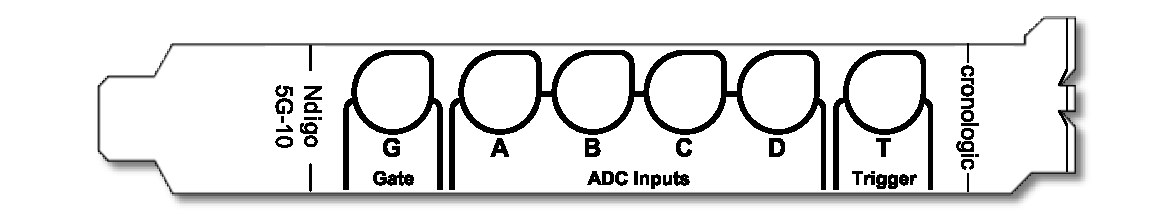
\includegraphics[width=0.6\textwidth]{figures/Ndigo-Slotblende.pdf}
			\caption{Input connectors of an Ndigo5G located on the PCI bracket.}
		\end{center}
	\end{figure*}
	%
	\begin{figure*}[ht]
		\begin{center}
			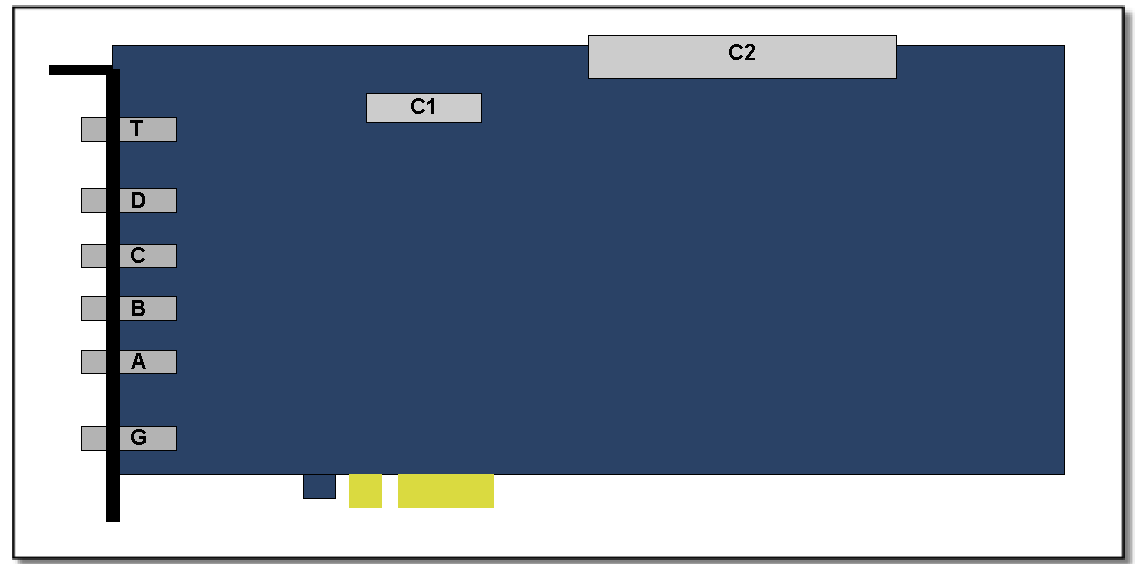
\includegraphics[width=0.7\textwidth]{figures/Ndigo_schematic.pdf}
			\caption{Schematics of an Ndigo5G board showing inter-board connectors C1 and C2.\label{fig:schematics}}
		\end{center}
	\end{figure*}
%
	\subsection{Analog Inputs}
	%
		\begin{figure*}[hb]
			\begin{center}
				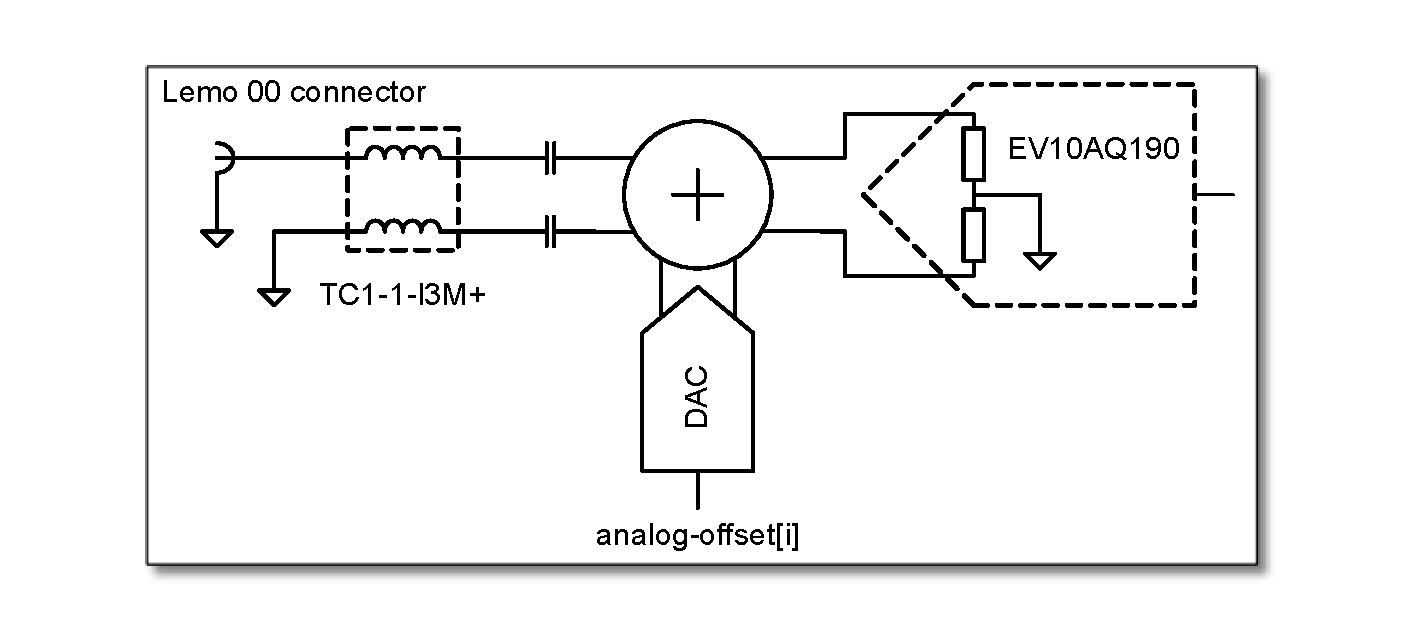
\includegraphics[width=0.8\textwidth]{figures/InputCircuit.pdf}
				\caption{Input circuit for each of the four analog channels.}
			\end{center}
		\end{figure*}
		%
		The analog inputs of the ADC are single ended LEMO00 coax connectors. The inputs have a $50\Omega$ impedance and are AC coupled. The inputs are converted to a differential signal using a balun.
		%
		\subsubsection{Analog Offsets}
		%
			\begin{figure*}[ht]
				\begin{center}
					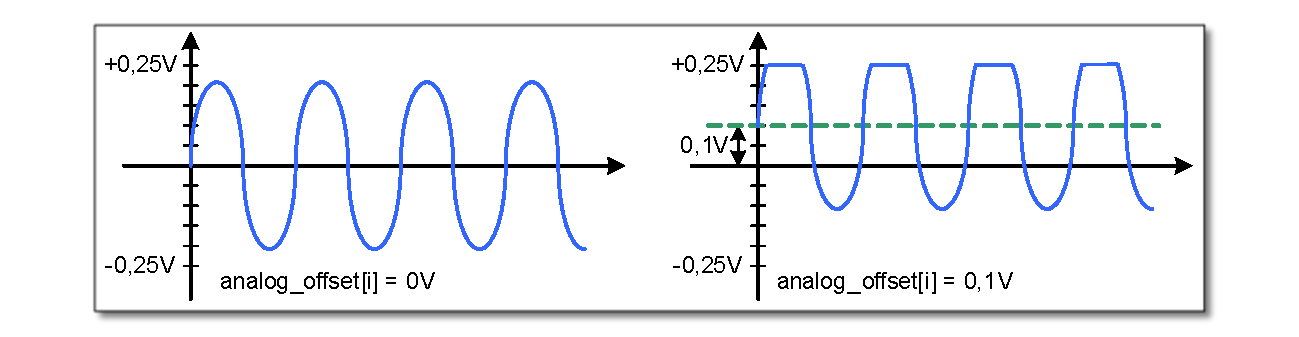
\includegraphics[width=\textwidth]{figures/AnalogOffset_Sine.pdf}
					\caption{Users can add analog offset to the input before sampling}
				\end{center}
			\end{figure*}	
			%
			AC coupling removes the common mode voltage from the input signal. Users can move the common mode voltage to a value of their choice using the analog\tu offset parameter of each channel before sampling.\par
			%
			\begin{figure*}[!ht]
				\begin{center}
					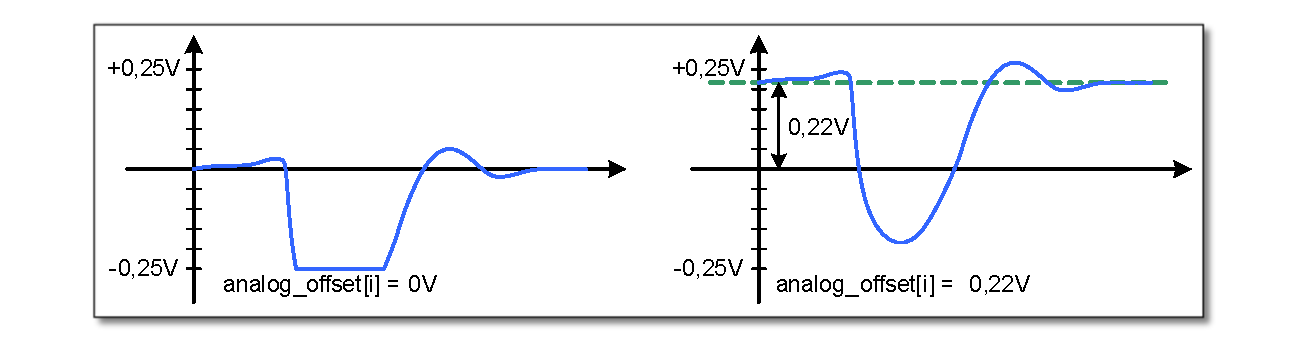
\includegraphics[width=\textwidth]{figures/AnalogOffset_Pulse.pdf}
					\caption{Asymmetric signal shifted to increase dynamic range\label{fig:shiftInput}}
				\end{center}
			\end{figure*}	
			%
			This feature is useful for highly asymmetric signals, such as pulses from TOF spectrometers or LIDAR systems. Without analog offset compensation, the pulses would begin in the middle of the ADC range, effectively cutting the dynamic range in half (see Figure \ref{fig:shiftInput}). By shifting the DC baseline to one end of the ADC range, the input range can be used fully, providing the maximum dynamic range. The analog offset can be set between $\pm 0,25V$.
		%
	\subsection{Digital Inputs}
	
		There are two digital inputs on the front slot cover called Trigger and Gate.\par
		Both inputs provide a digital input signal routed to the trigger matrix. These signals can be used to trigger any of the trigger state machines and gating blocks. The inputs are AC coupled. DC offset is configurable via the \textsf{dc\tu offset} parameter in the configurations structure to support positive and negative input pulses. \textsf{dc\tu offset[1]} is the offset for the Trigger input and \textsf{dc\tu offset[0]} is the offset for the GATE input.\par
		The configuration is set via the structures \textsf{trigger\allowbreak [NDIGO\tu TRIGGER\tu TRIGGER]} for the Trigger input and \textsf{trigger[NDIGO\tu TRIGGER\tu GATE]} for the GATE input. The input circuit is shown in Figure \ref{fig:DigitalInput} on page \pageref{fig:DigitalInput}.
		
		\subsubsection{TDC on Trigger Input}
		
			There is a TDC connected to the Trigger input. When used with the TDC, the Trigger input supports negative pulses only . The TDC creates packets of type 8. These packets first contain a coarse timestamp and a payload that can be used to calculate the trigger position with higher precision. The function \textsf{ndigo\tu process\tu tdc\tu packet()} can be used to replace the coarse timestamp with the precise timestamp. This function is described in section \ref{cp:readout} on page \pageref{cp:readout}.
			TDC pulses must have a minimum duration of 3.3ns. The dead-time of the TDC is 32ns.

			\textsf{NDIGO\tu TRIGGER\tu TDC} is an alias for \textsf{NDIGO\tu TRIGGER\tu TRIGGER}.


\section{Extension Card\label{cp:extcard}}

	The Ndigo Extension card provides additional inputs or outputs to the FPGA. It is connected to the Samtec QSS-025 connector on an Ndigo5G by an Samtec SQCD cable assembly.\par
	The Ndigo Extension Card provides up to ten single ended LEMO00 connectors. The circuit connecting to each of these circuits can be chosen to provide inputs or outputs. These can be AC or DC coupled. AC coupled inputs support NIM signaling.\par 
	The signals connect to 2.5V IO Pins of the Xilinx Virtex-5 FPGA. The current firmware revision provides the following signal connections:\par
	
	\begin{small}
	\begin{center}
		\begin{tabular}{|c|c|c|c|c|}
			\hline
			Connector & QSS Pin & FPGA Pin & Direction & Signal\\
			\hline\hline
			LEMO00: CH0 & 22 & AD9 & Input & Ndigo Extension digital channel 0\\\hline
			LEMO00: CH1 & 18 & AE10 & Input & Ndigo Extension digital channel 1\\\hline
			LEMO00: CH2 & 14 & D10 & - & not connected\\\hline
			LEMO00: CH3 & 10 & AF9 & Output & 39 MHz clock for HPTDC\\\hline
			LEMO00: CH4 & 6 & AD11 & Output & 39 MHz clock for HPTDC\\\hline
			LEMO00: CH5 & 5 & AE7 & Output & 39 MHz clock for HPTDC\\\hline
			LEMO00: CH6 & 9 & AF7 & Output & 39 MHz clock for HPTDC\\\hline
			LEMO00: CH7 & 13 & D9 & - & not connected\\\hline
			LEMO00: CH8 & 17 & V9 & Input & Ndigo Extension digital channel 2\\\hline
			LEMO00: CH9 & 21 & W9 & Input & Ndigo Extension digital channel 3\\\hline
			SYNC1: Sync-TDC8 & 26 & F9 & - & not connected\\\hline
			SYNC1: Sync-HPTDC & 44 & AA7 & Output & Sync for HPTDC\\\hline
		\end{tabular}
	\end{center}
	\end{small}
	
	The 4 digital inputs are routed to the bus inputs of the trigger matrix to be used for triggering. The routing can be configured to either ORing the sync bus and extension channels or use the extension channels exclusively.

	\begin{center}
		\begin{tabular}{|c|c|c|c|}
			\hline
			Connector & Extension Card & Trigger matrix input  & Trigger matrix input\\
			& Digital Channel & ignore\tu cable = 0 & ignore\tu cable = 1\\
			\hline\hline
			LEMO00: CH0 & 0 & BUS0 = EXT0 \textbar\ Sync Cable 0 & BUS0 = EXT0\\\hline
			LEMO00: CH1 & 1 & BUS1 = EXT1 \textbar\ Sync Cable 1 & BUS1 = EXT1\\\hline
			LEMO00: CH8 & 2 & BUS2 = EXT2 \textbar\ Sync Cable 2 & BUS2 = EXT2\\\hline
			LEMO00: CH9 & 3 & BUS3 = EXT3 \textbar\ Sync Cable 3 & BUS3 = EXT3\\\hline
		\end{tabular}
	\end{center}

\section{Ndigo5G Functionality}
	\subsection{ADC Modes}
	
		Depending on board configuration, the analog input signal is quantized to 8 or 10 bits. However, the board always scales and offsets the data to 16 bit signed data centered around 0.\par
		Data processing such as trigger detection or packet building are always performed on 3.2ns intervals. Depending on the ADC mode, this interval may contain 4, 8 or 16 samples.\par
		The board supports using one, two or four channels:
		
		\subsubsection{1 Channel Modes A, B, C and D}
		
			In these modes, only a single channel is used. The analog signal on that channel is digitized at 5Gsps. Packet size is always a multiple of 16 samples per 3.2ns. See Figure \ref{fig:1ChannelMode} on page \pageref{fig:1ChannelMode} and Figure \ref{fig:1ChannelTriggering} on page \pageref{fig:1ChannelTriggering}.		
		
		\subsubsection{2 Channel Modes AC, BC, AD and BD}
		
			In these modes, two channels are used simultaneously. The analog signals on these channels are digitized at 2.5Gsps each. Packet size is always a multiple of 8 samples per 3.2ns. See Figure \ref{fig:2ChannelMode} on page \pageref{fig:2ChannelMode} and Figure \ref{fig:2ChannelTriggering} on page \pageref{fig:2ChannelTriggering}.			
		
		\subsubsection{4 Channel Mode ABCD}
		
			In this mode, all four channels are digitized independently at 1.25Gsps each. The packet size is always a multiple of 4 samples per 3.2ns. See Figure \ref{fig:4ChannelMode} on page \pageref{fig:4ChannelMode} and Figure \ref{fig:4ChannelTriggering} on page \pageref{fig:4ChannelTriggering}.		
		
		\subsubsection{Multiple Sampling Modes AAAA, BBBB, CCCC and DDDD}
		
			In these modes, only one analog input channel is used, but the channel is sampled independently and simultaneously by four ADCs at 1.25Gsps. The board creates four independent streams with 4 samples each per 3.2ns.\par
			Using the same trigger setting on all ADCs, can be used to reduce noise by averaging the four channels. To deal with complex triggering conditions, different trigger settings on each of the ADCs can be used.\par
			The Ndigo5G provides 4 ADCs sampling at 1.25Gsps each. Higher speed modes are implemented by interleaving two or four of these ADCs.\par
			During interleaving, the Ndigo5G firmware reorders and groups the data into a linear sample stream. The process is fully transparent. For users, the only difference is that a 3.2ns cycle can contain 4, 8 or 16 samples, depending on mode.
		
		\begin{figure*}[hb]
			\begin{center}
				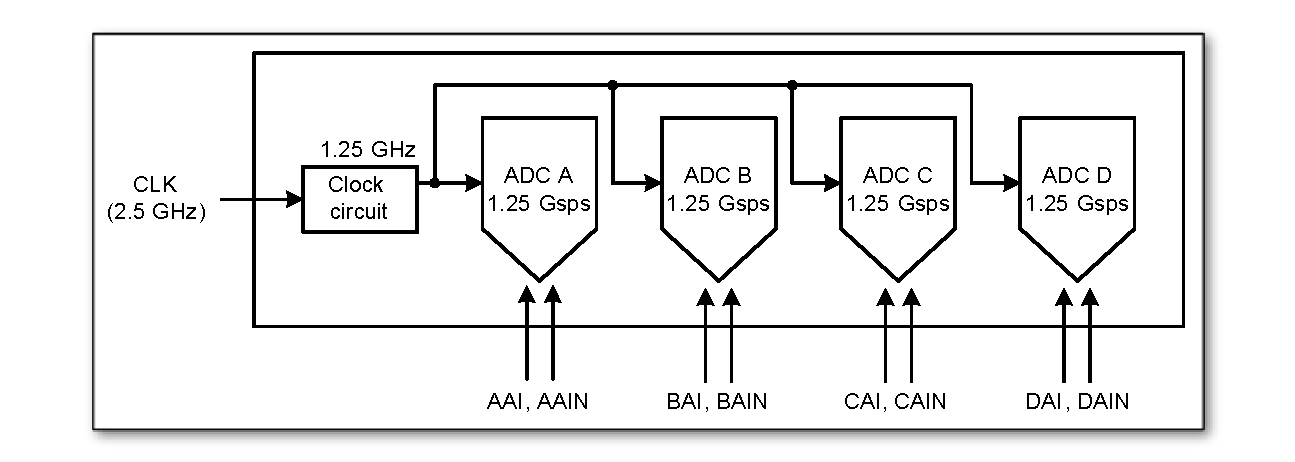
\includegraphics[width=\textwidth]{figures/4ChannelMode.pdf}
				\caption{ADCs in 4 channel mode ABCD at 1.25Gsps.\label{fig:4ChannelMode}}
			\end{center}
		\end{figure*}
		
		\begin{figure*}[ht]
			\begin{center}
				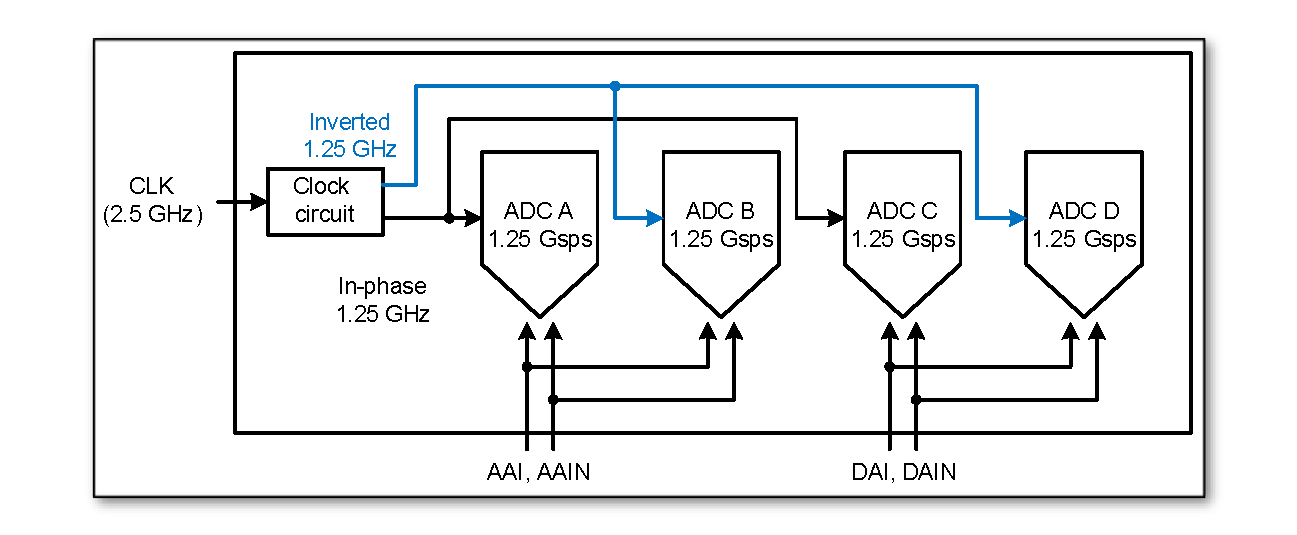
\includegraphics[width=\textwidth]{figures/2ChannelMode.pdf}
				\caption{ADCs in 2 channel mode AD, interleaved for 2.5Gsps.\label{fig:2ChannelMode}}
			\end{center}
		\end{figure*}		
		
		\begin{figure*}[hb]
			\begin{center}
				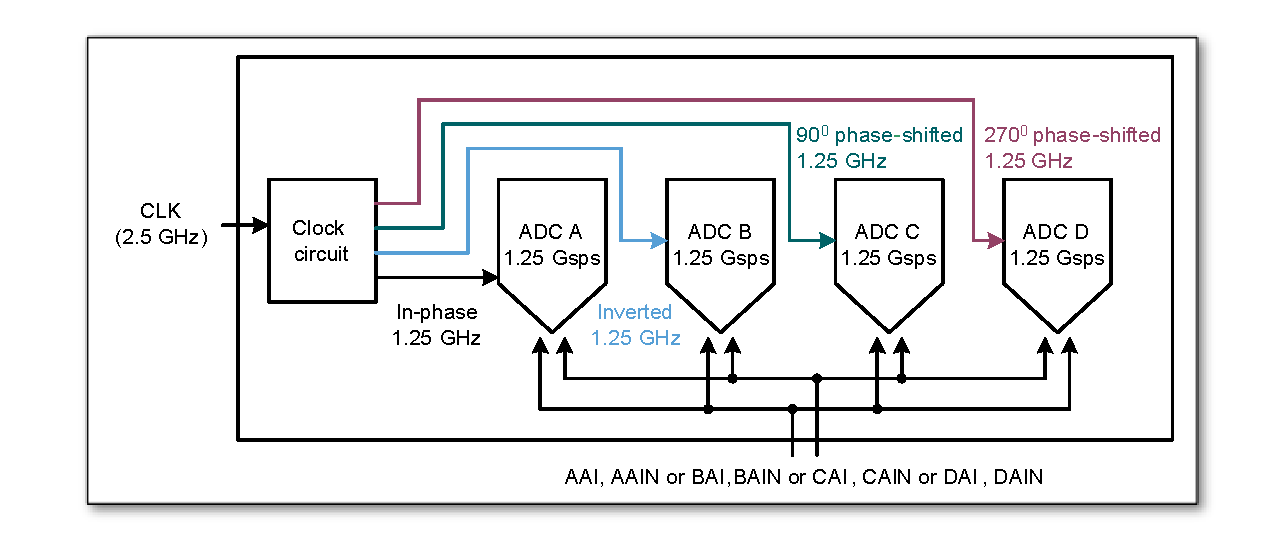
\includegraphics[width=\textwidth]{figures/1ChannelMode.pdf}
				\caption{ADCs in 1 channel mode A, B, C or D interleaved for 5Gsps.\label{fig:1ChannelMode}}
			\end{center}
		\end{figure*}
		
	\subsection{Zero Suppression}
	
		One of Ndigo5G's key features is on-board zero suppression to reduce PCIe bus load. Only data that passes specifications predefined by the user is transmitted. This guide refers to transmitted waveform data as ``packets''. A packet contains the waveform data and a timestamp giving the absolute time (i.e. the time since start of data acquisition) of the packet's last sample.\par
Figure \ref{fig:ZeroSupp} shows a simple example: Data is written to the PC only if values exceed a specified threshold. Expanding on that, Ndigo5G's zero suppression can be used to realize much more complex scenarios.

		\begin{figure*}[hb]
			\begin{center}
				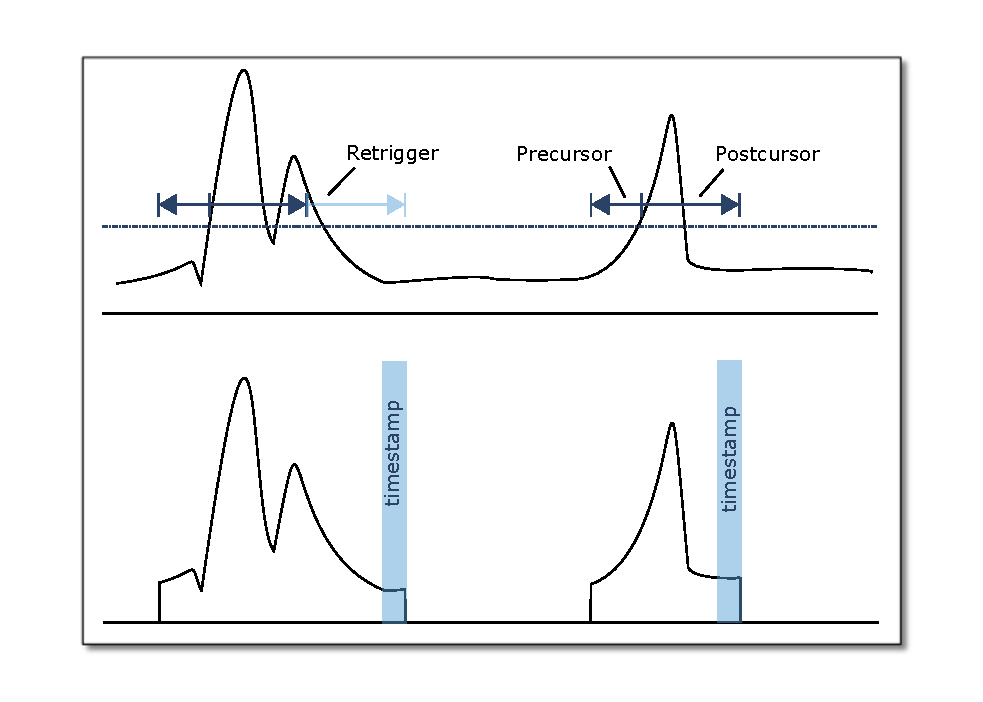
\includegraphics[width=0.8\textwidth]{figures/ZeroSupp.pdf}
				\caption{Simple zero suppression: Only data with values above a threshold are
written to the PC.\label{fig:ZeroSupp}}
			\end{center}
		\end{figure*}
	
	\subsection{Trigger Blocks}
	
		Ndigo5G-10 and Ndigo5G-8 record analog waveforms using zero suppression. Whenever a relevant waveform is detected, data is written to an internal FIFO memory. Each ADC channel has one trigger block determining whether data is written to the FIFO. The parameters are set in  Structure \textsf{ndigo\tu trigger\tu block}(See chapter \ref{cp:triggerblock} on page \pageref{cp:triggerblock}).\par
		
		Each trigger block consists of two independent units that check the incoming raw data stream for trigger conditions (Fig. \ref{fig:ZeroSupp} on page \pageref{fig:ZeroSupp}). Users can specify a threshold and can choose whether triggering is used whenever incoming data is below or above the threshold (level triggering) or only if data exceeds the threshold (edge triggering).\par

		A gate length can be set to extend the trigger window by multiples of 3.2ns. Furthermore, if users choose precursor values $> 0$, the trigger unit will start writing data to the FIFO $\text{precursor}\cdot 3.2ns$ before the trigger event.\par

		When using edge triggering, all packets have the same length (Figure \ref{fig:edge-trigger} on page \pageref{fig:edge-trigger}): $\text{precursor}+\text{length}+1$ cycles of 3.2ns. For level triggering, packet length is data dependent (Figure \ref{fig:level-trigger} on page \pageref{fig:level-trigger}).\par

		Please note that triggering is not accurate to sample. For each 3.2ns clock cycle, it is determined whether on any sample during that clock cycle a trigger condition is met. The clock cycle is then selected as the trigger point. As a result, the trigger sample can be anywhere within a range of up to 16 samples in single channel mode (Figure \ref{fig:1ChannelTriggering} on page \pageref{fig:1ChannelTriggering}) at 16 samples per 3.2ns.\par

		If retriggering is active, the current trigger window is extended if a trigger event is detected inside the window.\par

		A trigger block can use several input sources:

		\begin{itemize}
			\item the 8 trigger decision units of all four ADC channels (Figure \ref{fig:analog-trigger} on page \pageref{fig:analog-trigger})
			\item the GATE input (Figure \ref{fig:DigitalInput} on page \pageref{fig:DigitalInput})
			\item the Trigger or TDC input,  (Figure \ref{fig:DigitalInput} on page \pageref{fig:DigitalInput})
			\item a function trigger providing random or periodic triggering (Section \ref{cp:AutoTriggeringFunctionGenerator} on page \pageref{cp:AutoTriggeringFunctionGenerator})
			\item triggers originating from other cards connected with the sync cable or from the Ndigo Extension card (BUS0, BUS1, BUS2, BUS3)
			\item A second set of trigger units with names ending in \textsf{\tu pe} for the digital inputs Trigger, GATE, BUS0, BUS1, BUS2, and BUS3 configured for positive edge triggering. Together with the regular trigger units on this inputs, both edges of a pulse can be used in the trigger logic. This set of triggers is not available as inputs for the gate blocks.
		\end{itemize}

		Trigger inputs from the above sources can be concatenated using logical ``OR'' (Figure \ref{fig:triggermatrix} on page \pageref{fig:triggermatrix}) by setting the appropriate bits in the trigger blocks source mask.\par
		
Triggers can be fed into the gate blocks described on page \pageref{fig:GatingBlock} (Figure \ref{fig:GatingBlock}). Gate blocks can be used to block writing data to the FIFO. That way, only zero suppressed data occurring when the selected gate is active is transmitted. This procedure reduces PCIe bus load even further (Figure \ref{fig:GatingBlock}).

		\begin{figure*}[ht]
			\begin{center}
				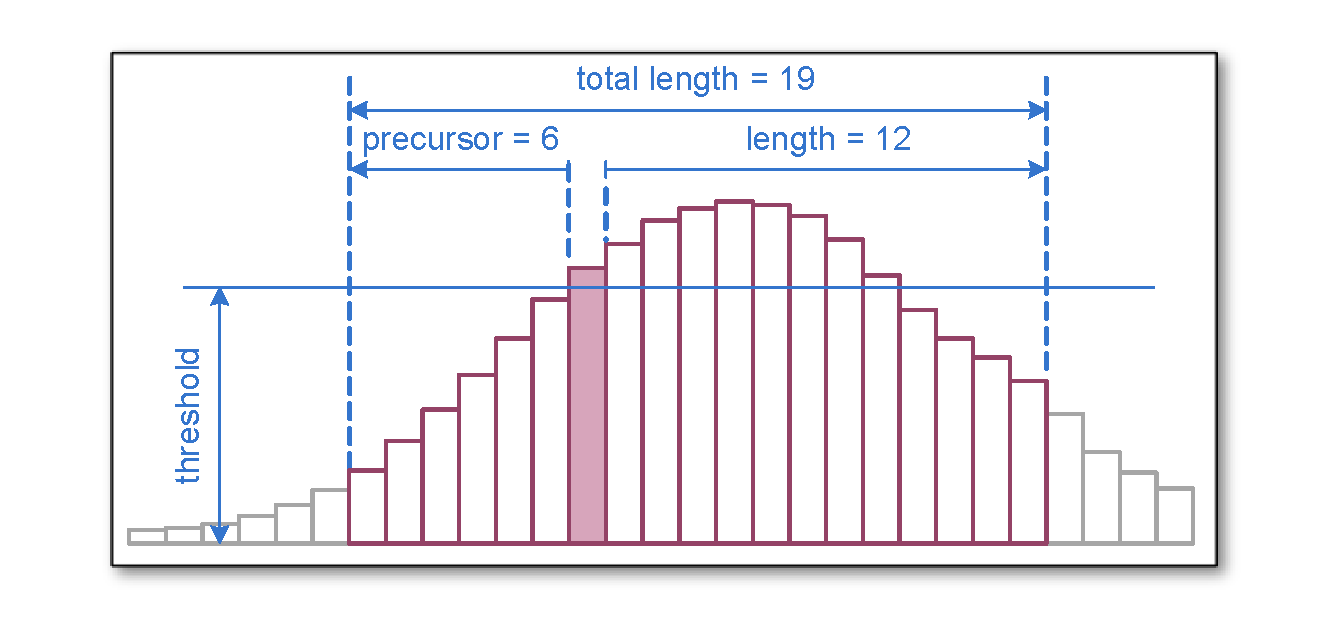
\includegraphics[width=0.8\textwidth]{figures/edge-trigger.pdf}
				\caption{Parameters for edge triggering\label{fig:edge-trigger}}
			\end{center}
		\end{figure*}
		
		\begin{figure*}[hb]
			\begin{center}
				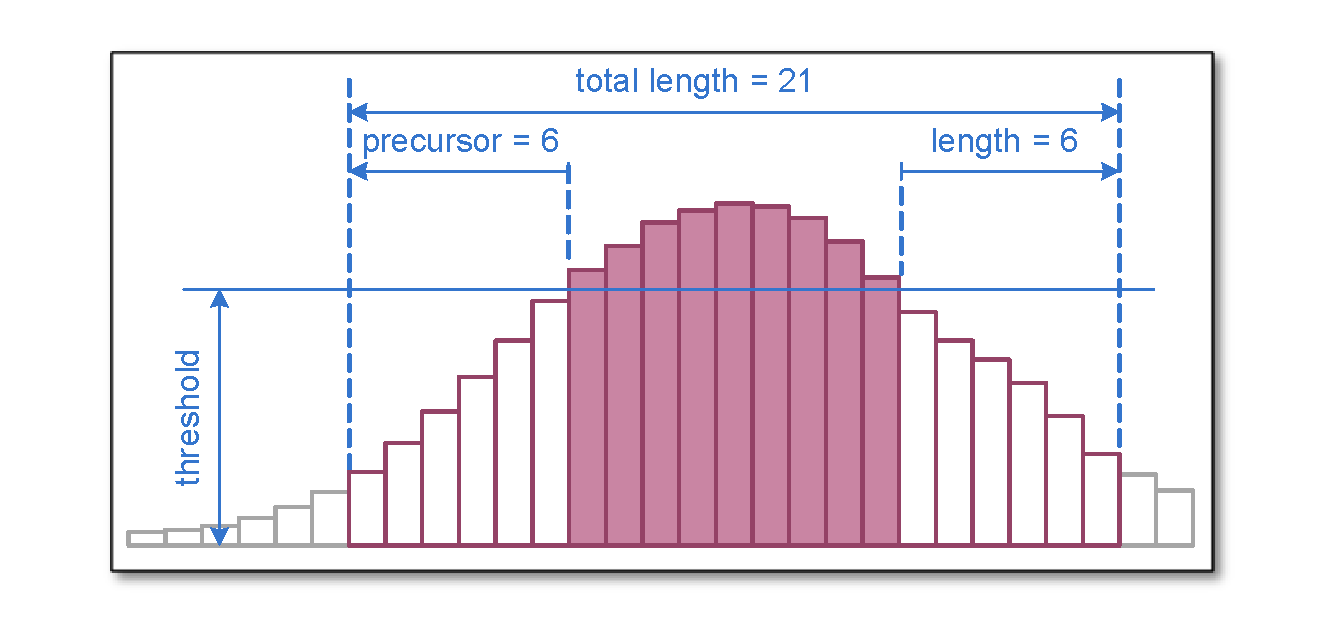
\includegraphics[width=0.8\textwidth]{figures/level-trigger.pdf}
				\caption{Parameters for level triggering\label{fig:level-trigger}}
			\end{center}
		\end{figure*}
	
		\begin{figure*}[ht]
			\begin{center}
				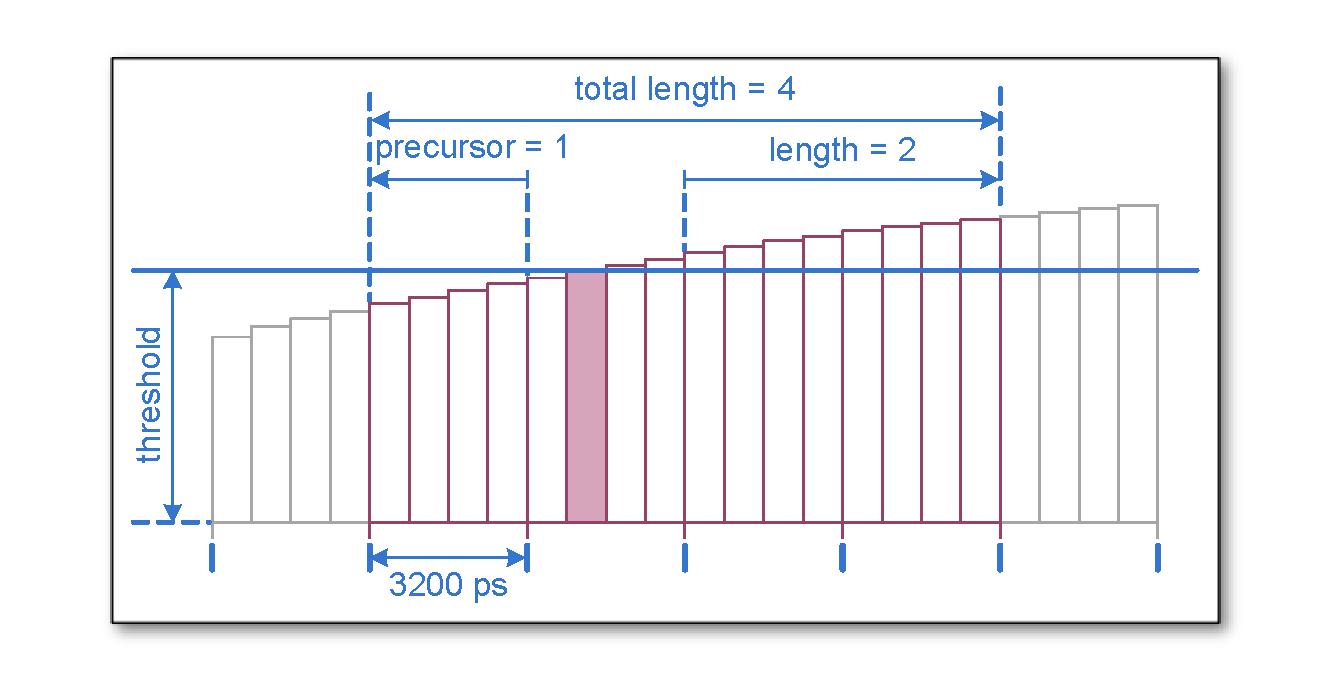
\includegraphics[width=0.8\textwidth]{figures/4ChannelTriggering.pdf}
				\caption{Triggering in 4 channel mode at 4 samples per clock cycle.\label{fig:4ChannelTriggering}}
			\end{center}
		\end{figure*}
	
		\begin{figure*}[hb]
			\begin{center}
				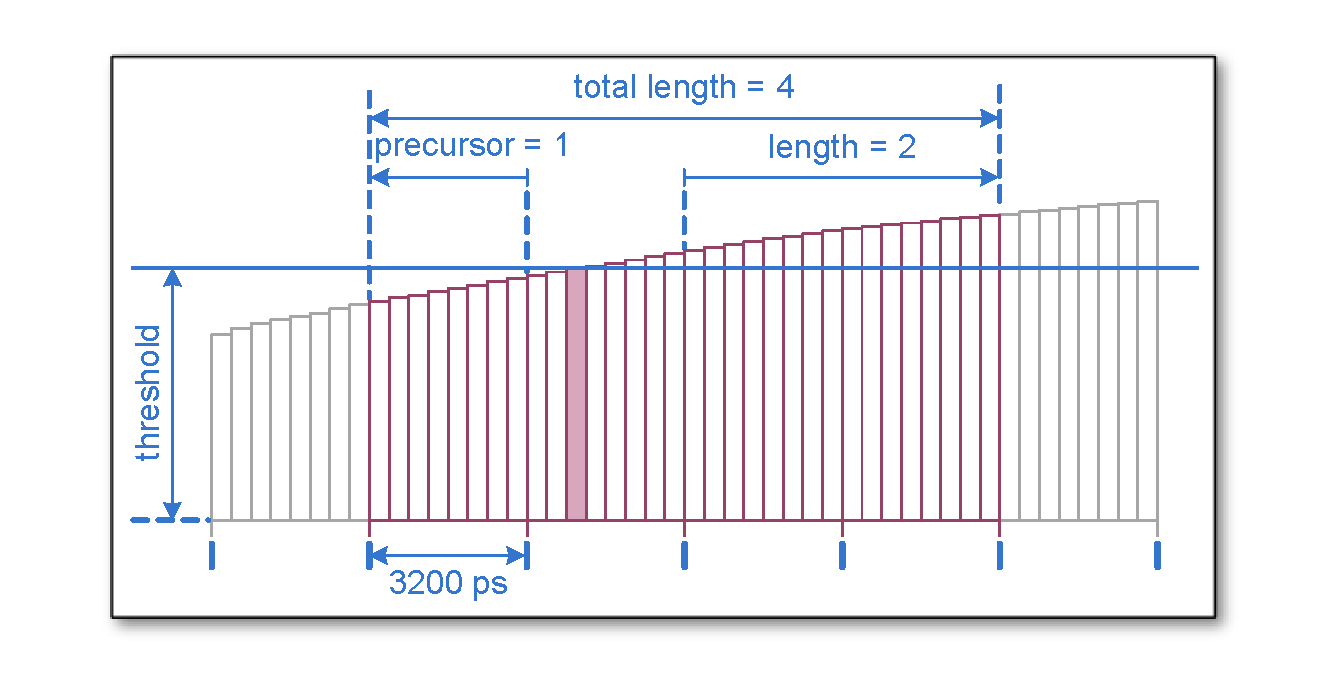
\includegraphics[width=0.8\textwidth]{figures/2ChannelTriggering.pdf}
				\caption{Triggering in 2 channel mode at 8 samples per clock cycle.\label{fig:2ChannelTriggering}}
			\end{center}
		\end{figure*}
	
		\begin{figure*}[ht]
			\begin{center}
				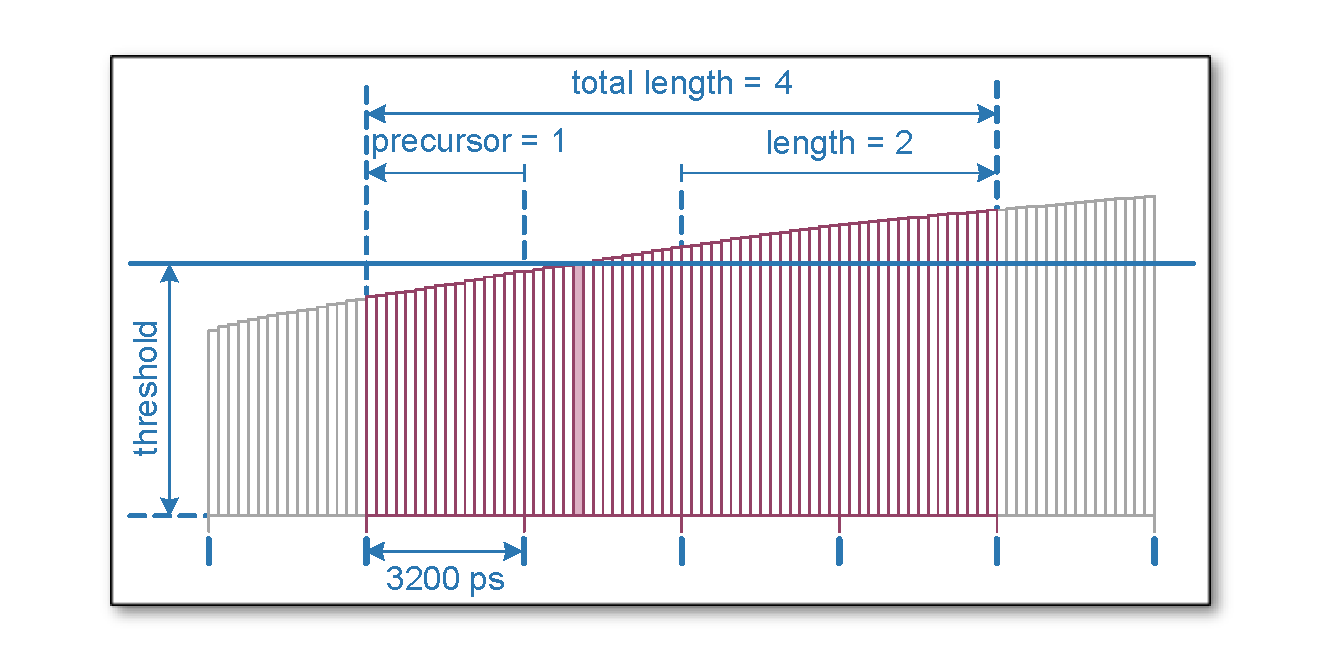
\includegraphics[width=0.8\textwidth]{figures/1ChannelTriggering.pdf}
				\caption{Triggering in 1 channel mode at 16 samples per clock cycle.\label{fig:1ChannelTriggering}}
			\end{center}
		\end{figure*}
		
		\begin{figure*}[hb]
			\begin{center}
				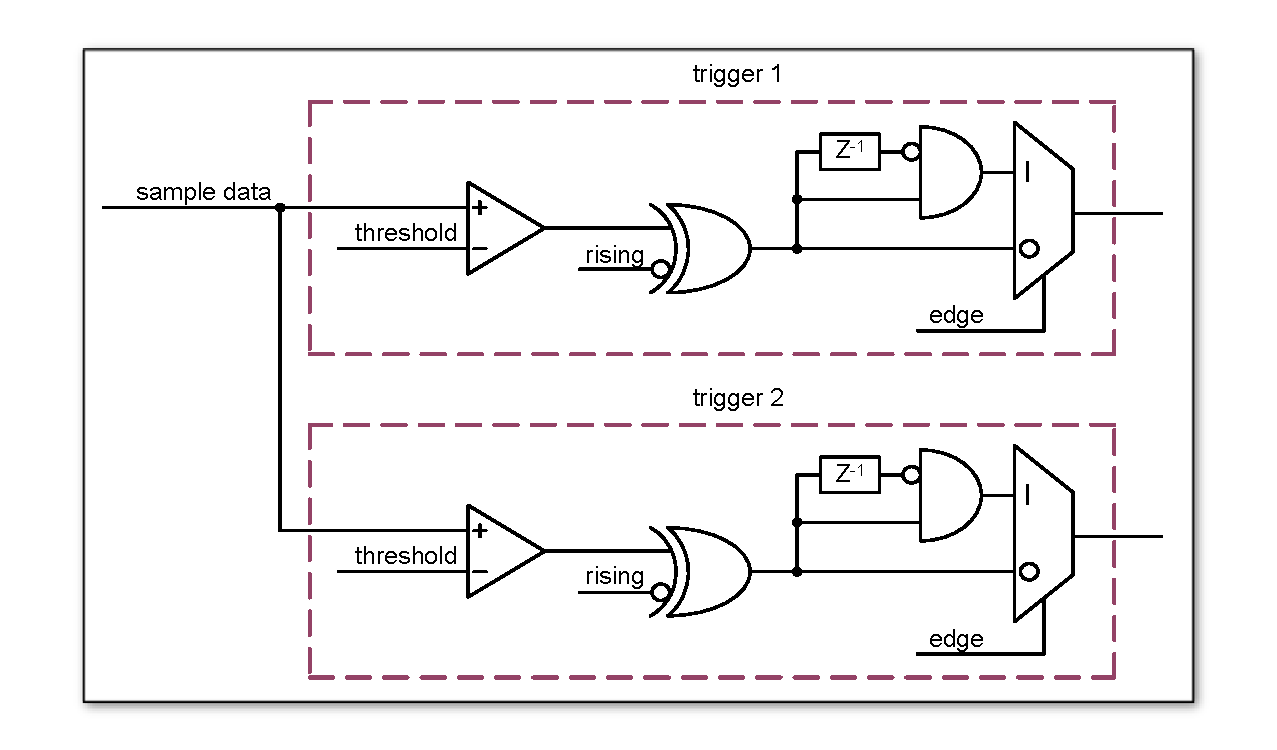
\includegraphics[width=0.8\textwidth]{figures/analog-trigger.pdf}
				\caption{From the ADC inputs, a trigger unit creates an input flag for the trigger matrix. Each digitizer channel (A, B, C, D) has two trigger units.\label{fig:analog-trigger}}
			\end{center}
		\end{figure*}
	
		\begin{figure*}[ht]
			\begin{center}
				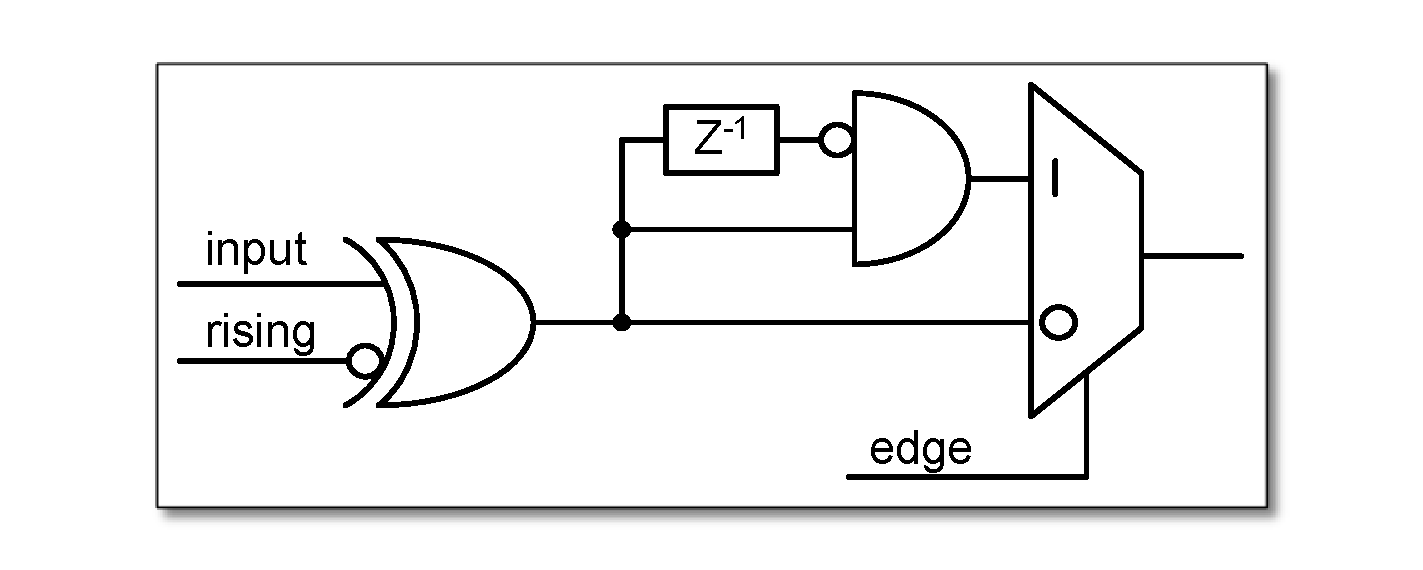
\includegraphics[width=0.5\textwidth]{figures/DigitalInput.pdf}
				\caption{The digital inputs Trigger, GATE, BUS0, BUS1, BUS2 and BUS3 have simpler trigger units.\label{fig:DigitalInput}}
			\end{center}
		\end{figure*}
		
		\begin{figure*}
			\begin{center}
				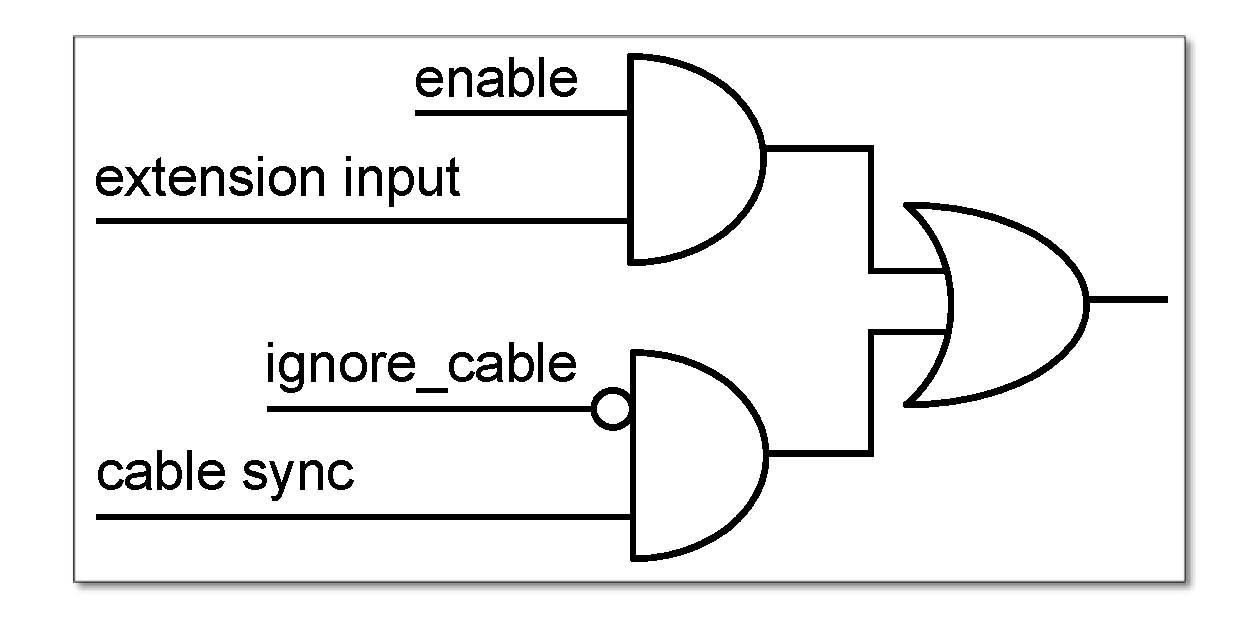
\includegraphics[width=0.5\textwidth]{figures/ExtensionBlock.pdf}
				\caption{\label{fig:ExtensionBlock} The extension block combines signals from the optional extension board and the sync cable.}
			\end{center}
		\end{figure*}
		
		\begin{figure*}
			\begin{center}
				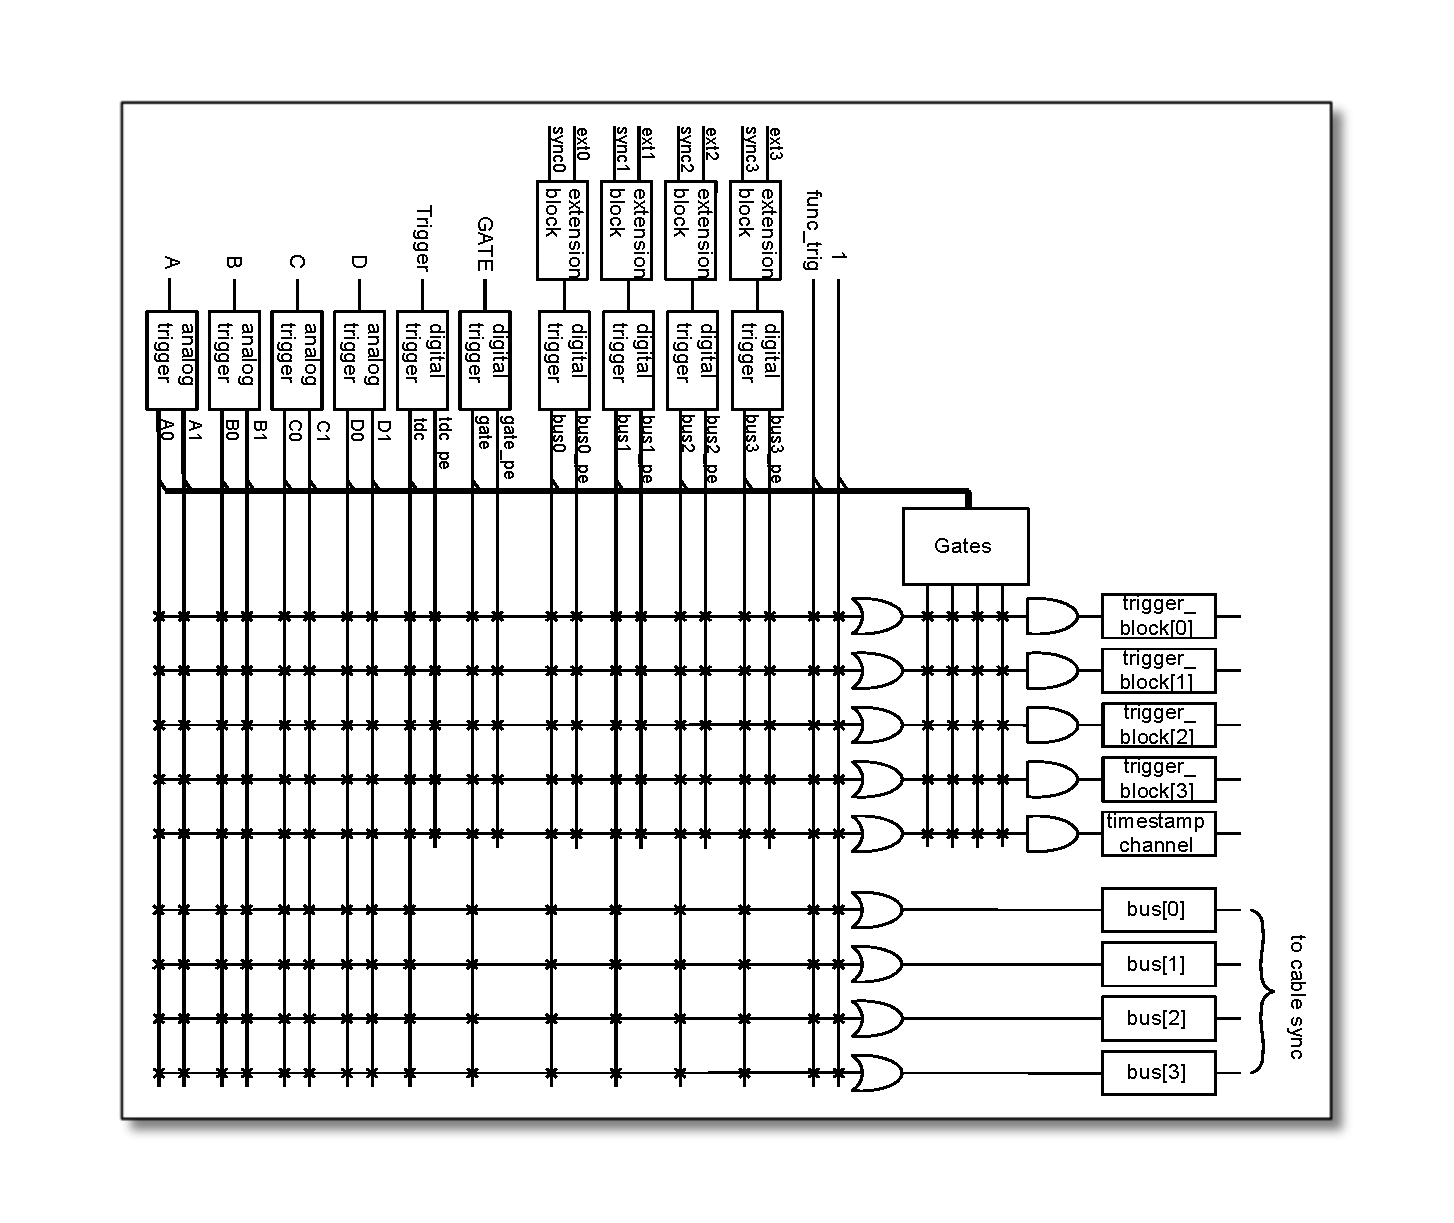
\includegraphics[width=\textwidth]{figures/triggermatrix.pdf}
				\caption{Trigger Matrix: The trigger signals of each ADC channel, the Triggerinput, the GATE input or the sync cable can be combined to create a trigger input for each trigger block.
The four gate signals can be used to suppress triggers during certain time frames.\label{fig:triggermatrix}}
			\end{center}
		\end{figure*}
	
	\subsection{Gating Blocks}
		
		\begin{figure*}[ht]
			\begin{center}
				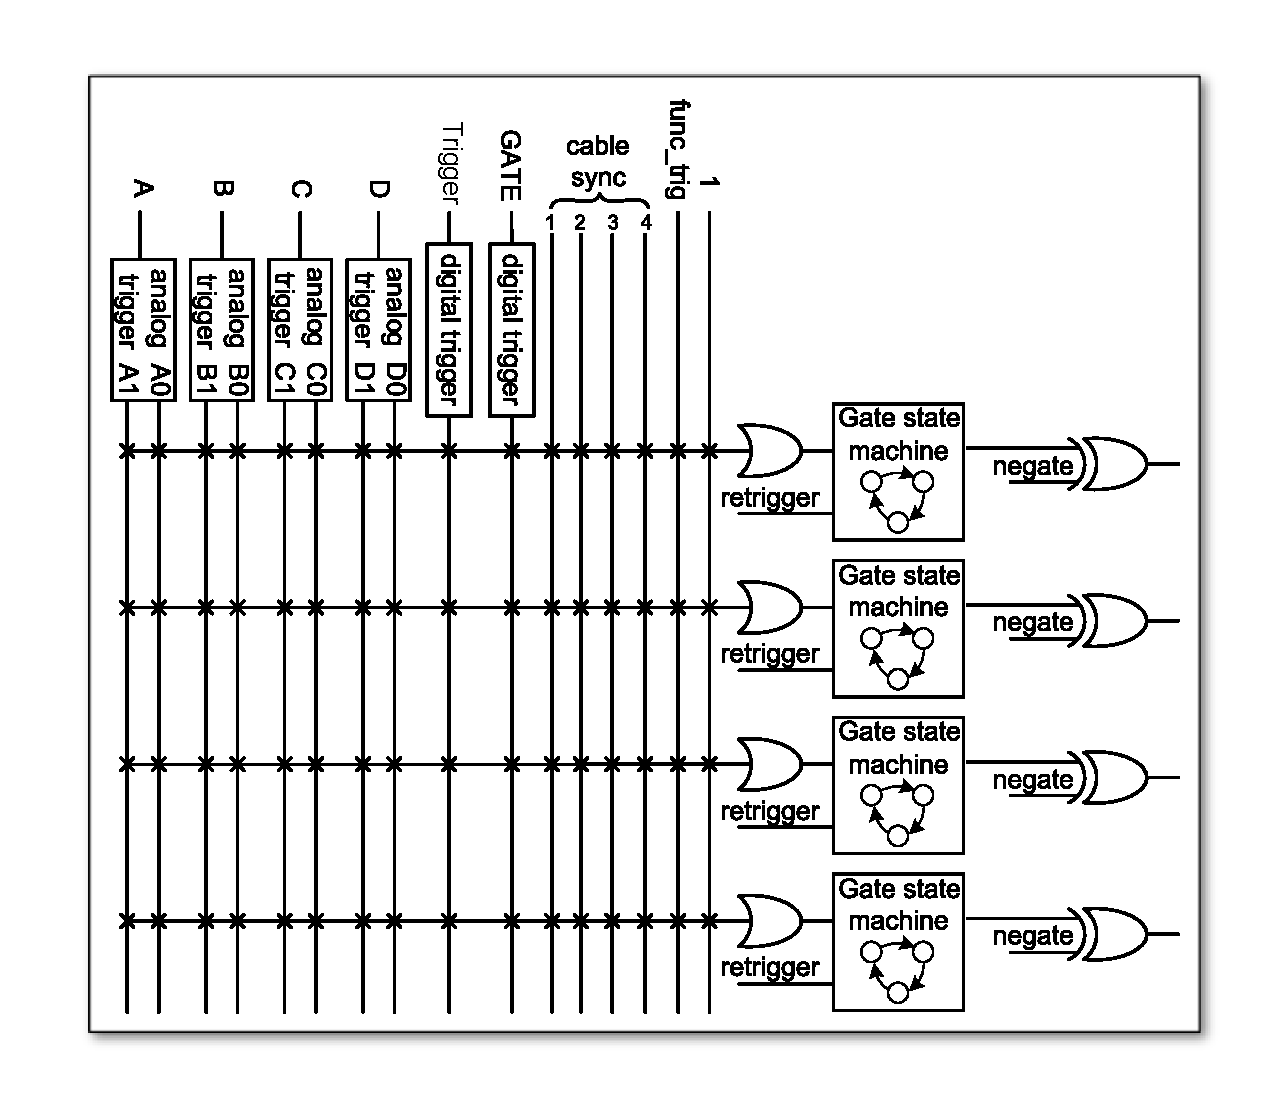
\includegraphics[width=0.8\textwidth]{figures/GatingBlocks.pdf}
				\caption{\label{fig:GatingBlock} Gating Blocks: Each gating block can use an arbitrary combination of inputs to trigger its state machine. The outputs can be individually inverted and routed to the AND-gate feeding the trigger blocks.}
			\end{center}
		\end{figure*}
		
		To decrease the amount of data transmitted to the PC, Ndigo5G includes 4 independent gate and delay units. A gate and delay unit creates a gate window starting at a specified time after a trigger, closing the window at gate stop. Both timing values — gate start and gate stop — must be set as 
multiples of 3.2ns.\par

		Trigger blocks can use the gate signal to suppress data acquisition: Only data that fulfills zero suppression specifications occurring in an active gate window is written to the PC.\par
		As input, any trigger from the 4 trigger blocks, the GATE and Trigger inputs, a trigger from a connected board and the function generator can be used.\par
		
		The retrigger feature will create a new gate if a trigger occurs during an active gate window. The gate signal can be inverted, causing an active gate to close for a time defined by the user.\par
		
		The parameters of a gating block are set in Structure \textsf{ndigo\tu gating\tu block} described on page \pageref{cp:gatingblock}.\par
		
		Figure \ref{fig:GateUDelay} shows the functionality of the gate timing and delay unit. Active gate time is marked in green.
		
		\begin{figure*}[ht]
			\begin{center}
				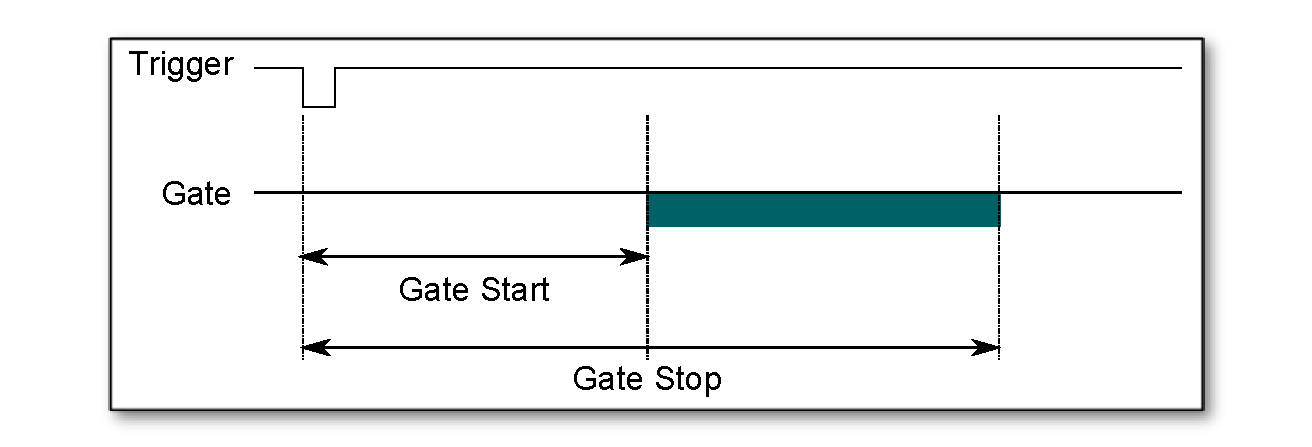
\includegraphics[width=0.8\textwidth]{figures/GateUDelay.pdf}
				\caption{\label{fig:GateUDelay} Gate and delay functionality: When a trigger occurs, the gate opens after a set period of time (``gate start'') and closes when it reaches ``gate stop''.}
			\end{center}
		\end{figure*}
		
		\subsubsection{Gating Example 1: Suppression of Noise After Starting an Acquisition}
			
			In mass spectrometer and other experiments, noise while starting data acquisition can result in undesired trigger events for that time period. To prevent noise in the output data, a gating block could be used to suppress all triggers during start-up.\par
			
			The following example illustrates the use of a gating block to prevent noise: The GATE input transmits a pulse on each acquisition start. The trigger structure of the GATE input is used to select pulse polarity. Then, the GATE trigger is selected as gating block input and the gating block's start parameter is set to 0. The stop parameter is set to the desired length measured in 3.2ns clock cycle and negate is set to true. The gating block will now output a low pulse of the desired length whenever there is a pulse on the GATE input.\par
			
		Enabling this gating block as an AND input to the trigger block, for which noise shall be suppressed.
			
		\subsubsection{Gating Example 2: Delayed Trigger}
		
			To sample a short window at a specified time after a trigger event on a channel, the gating block can be used to create a delayed trigger. To do this, one of the triggers of the channel of interested is configured to the desired parameters by selecting the threshold, setting the edge polarity and 
enabling edge triggering.\par

			Instead of directly using this trigger as input to the trigger block's input matrix, the trigger is selected as an input to a gating block. The block is configured to $start = delay$ [in 3.2ns clock cycles] 
and $stop = start+1$, $negate = false$. This causes the gating block to produce a one clock cycle pulse on its output after the specified delay.\par

			To send this pulse to the trigger block, the gating block must be enabled in the trigger block's AND matrix and the ONE trigger source must be selected. 
			
		\subsubsection{Gating Example 3: Dual Level Trigger}
		
			The gates provide AND connections between each other (see fig. \ref{fig:triggermatrix}) which can be used for example in a dual level trigger. For the acquisition of signal data with amplitudes between a lower and an upper bound, for example, two level triggers can be connected (see fig. \ref{fig:dualleveltrig}): a falling level trigger with an upper threshold and a rising level trigger with a lower threshold.\par
			Since the triggers are only connected by OR in the triggerblock logic (see fig. \ref{fig:triggermatrix}) they are assigned to one of the gates each and connected with AND via the gating block region of the trigger matrix (see fig. \ref{fig:triggermatrix} and \ref{fig:dualleveltriglogic}). Because of the dead times of the gates it is important to enable the retriggering feature. Furthermore a precursor of 2 clock cycles is needed, because the gates are delayed in relation to the ADC samples.\par
			\begin{figure*}[ht]
				\begin{center}
					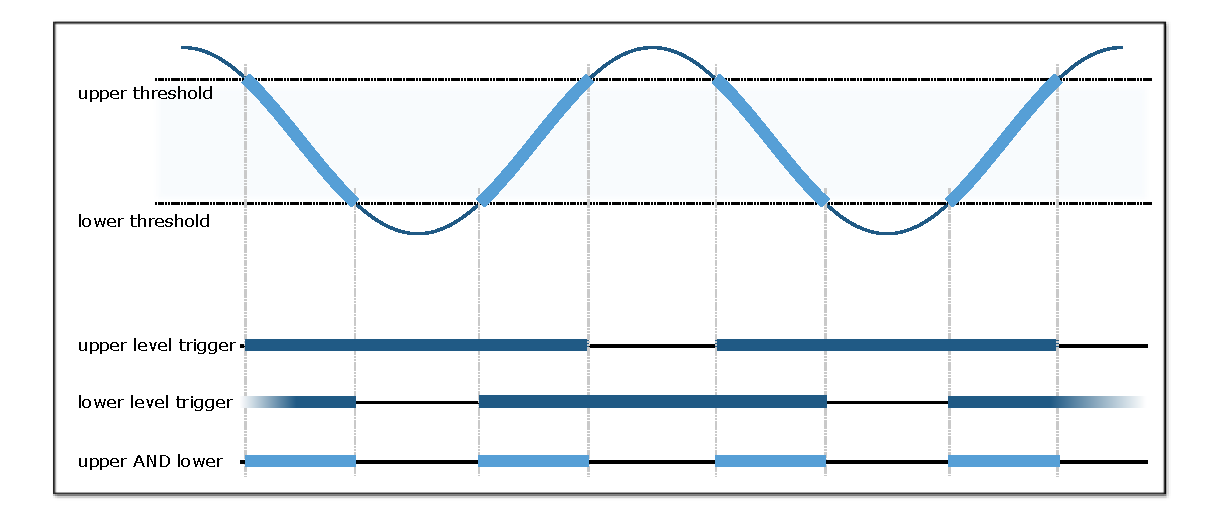
\includegraphics[width=\textwidth]{figures/dual_level_triggering.pdf}
					\caption{\label{fig:dualleveltrig}Measuring data with amplitude between an upper and a lower threshold by means of two level triggers.}
				\end{center}
			\end{figure*}	
			
			\begin{figure*}[ht]
				\begin{center}
					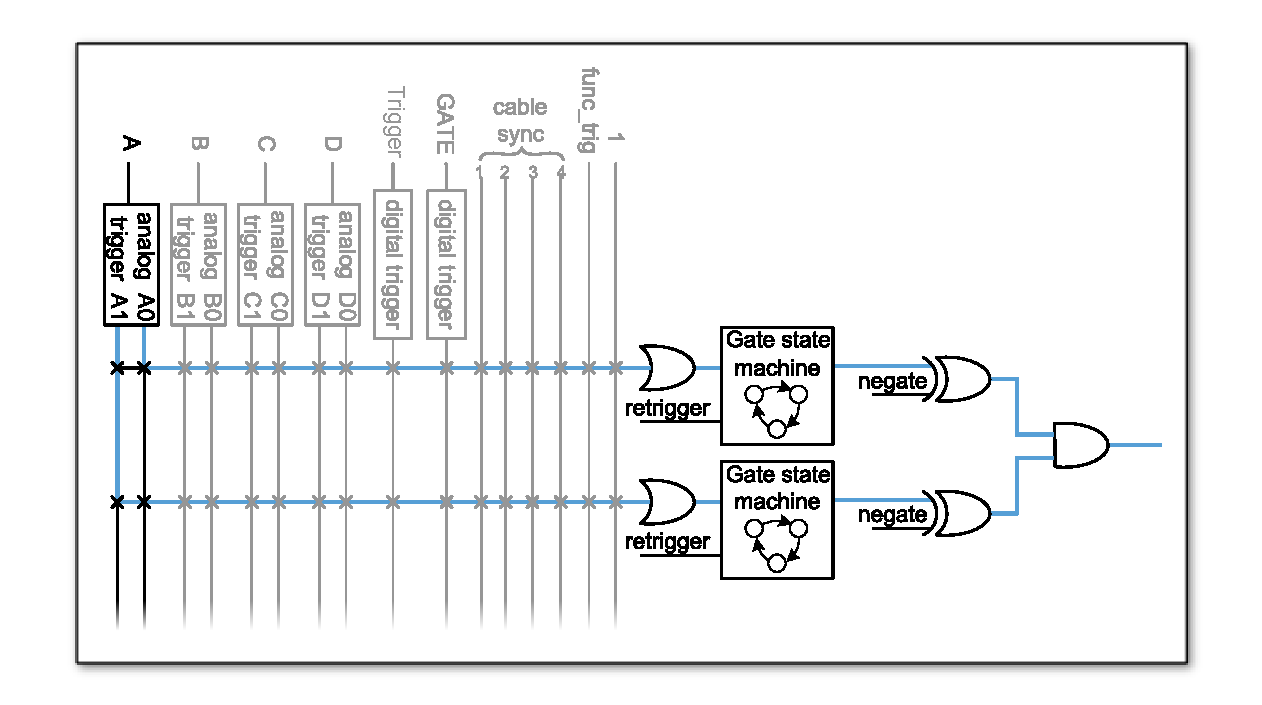
\includegraphics[width=\textwidth]{figures/dual-level-triggering_logic.pdf}
					\caption{\label{fig:dualleveltriglogic}Gating block logic for the AND connection of two triggers.}
				\end{center}
			\end{figure*}
			
			Config settings can be found in the following code snippet.
			
\lstset{
	language=[Visual]C++,
	keywordstyle=\bfseries\sffamily\color[rgb]{0,0,1},
	identifierstyle=\sffamily,
	commentstyle=\color[rgb]{0.133,0.545,0.133},
	stringstyle=\sffamily\color[rgb]{0.627,0.126,0.941},
	showstringspaces=false,
	basicstyle=\small,
	numberstyle=\footnotesize,
	numbers=left,
	stepnumber=1,
	numbersep=10pt,
	tabsize=2,
	breaklines=true,
	prebreak = \raisebox{0ex}[0ex][0ex]{\ensuremath{\hookleftarrow}},
	breakatwhitespace=false,
	aboveskip={1.5\baselineskip},
  columns=fixed,
  upquote=true,
  extendedchars=true,
% frame=single,
% backgroundcolor=\color{lbcolor},
}
\begin{lstlisting}[frame=tlrb]
	config.trigger_block[0].enabled = 1;
	config.trigger_block[0].precursor = 2;
	config.trigger_block[0].length = 0;
	config.trigger_block[0].sources = NDIGO_TRIGGER_SOURCE_ONE;
	config.trigger_block[0].gates = NDIGO_TRIGGER_GATE_0 | NDIGO_TRIGGER_GATE_1;
	config.gating_block[0].retrigger = 1;
	config.gating_block[0].stop = 0;
	config.gating_block[0].sources = NDIGO_TRIGGER_A0;
	config.gating_block[1].retrigger = 1;
	config.gating_block[1].stop = 0;
	config.gating_block[1].sources = NDIGO_TRIGGER_A1;
	config.trigger[NDIGO_TRIGGER_A0].rising = 0;
	config.trigger[NDIGO_TRIGGER_A0].threshold = 10000;
	config.trigger[NDIGO_TRIGGER_A1].rising = 1;
	config.trigger[NDIGO_TRIGGER_A1].threshold = -10000;
\end{lstlisting}
			
	\subsection{Auto Triggering Function Generator\label{cp:AutoTriggeringFunctionGenerator}}
	
		Some applications require periodic or random triggering. Ndigo5G's function generator provides this functionality.\par

		The delay between two trigger pulses of this trigger generator is the sum of two components: A fixed value M and a pseudo random value given by the exponent N. \par

		The period is

		\begin{align}
			T = 1 + M + [1...2^N]
		\end{align}

		clock cycles with a duration of 3.2 ns per cycle.\par
		
		This allows to monitor input signals at times the current trigger configuration does not trigger, e. g. to get base line information in mass spectrometry applications. It can also be used to determine a suitable threshold level for the trigger by first getting random statistics on the input signal.	
	
	\subsection{Timestamp Channel}

		The timestamp channel produces a stream of small packets that denote the time of the trigger event. An arbitrary set of trigger sources can be selected in the trigger matrix to cause the creation of a packet.\par
		
		The packets have a fixed length of 16 bytes. The format is described on page \pageref{cp:packetformat}. The length field of the packet contains a 32 bit pattern that contains the levels of all trigger sources at the time of the trigger event except for the period monitor. Only one packet is created, no matter how many trigger sources caused the timestamp channel to trigger.	
	
	\subsection{Data Lookup Table}
	
		In some applications it might be useful to modify the ADC sample data by a user defined function $f(x)$. In this case the onboard FPGA is able to perform this task such that the the data stream consists of data words $f(sample)$ instead of $sample$. The function f(x) is applied using a 1024 word lookup table (LUT) which needs to be provided by the user. This is done by defining the corresponding function as a custom\_lut-member of the ndigo\_configuration structure. Please feel free to contact cronologic if you plan the use this feature. The onboard INL correction is applied prior to mapping the LUT values.  
	
\section{Multiple Ndigo boards synchronization}
	Using several Ndigo devices in applications that use more channels than a single board can provide requires synchronized operation. To ensure exact synchronization, a delay parameter needs to be set for each board. This parameter might change in case boards are swapped, added or removed and in some cases might change after a firmware update.\par
	
	The calibration tool ``MultiboardCalibration.exe'' is available after installing the Ndigo device driver. It is used to find appropriate delay values for each board in a given board setup. After starting, the application lists all Ndigo boards found (Figure \ref{fig:SyncCalibTool}).\par

	\begin{figure*}[ht]
		\begin{center}
			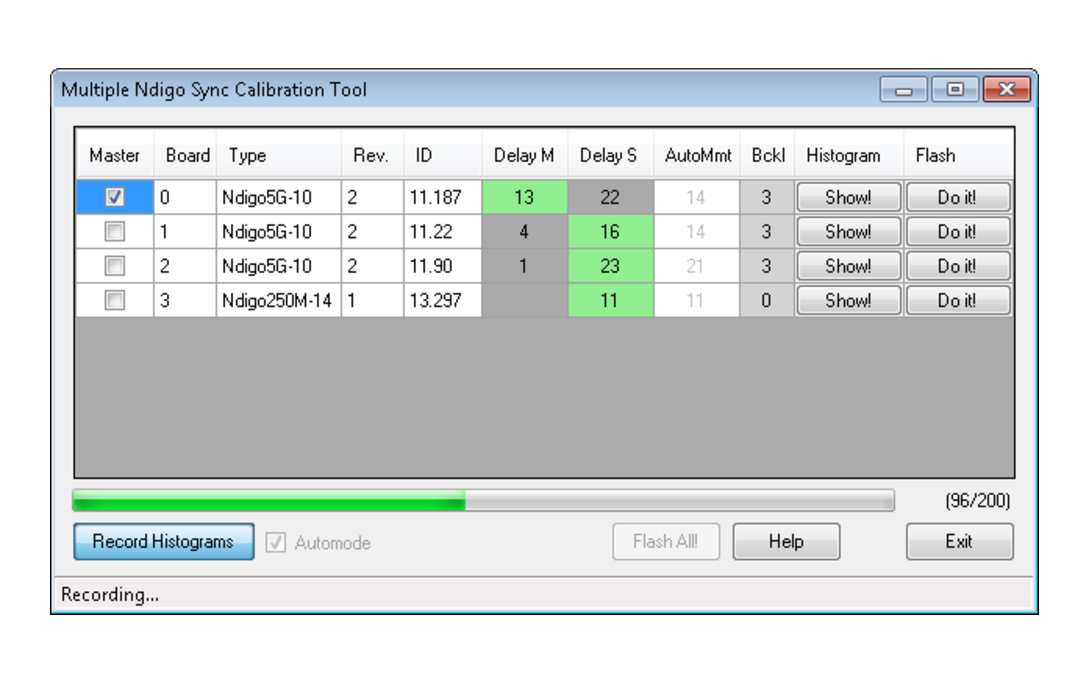
\includegraphics[width=0.7\textwidth]{figures/SyncCalibTool.pdf}
			\caption{Main window of the multiple boards sync calibration tool\label{fig:SyncCalibTool}}
		\end{center}
	\end{figure*}

	A board's appropriate delay depends on whether it operates in master or slave mode. The respective values can be set in the column ``Delay M'' (for master boards) and ``Delay S'' (for slave boards). The designated master board can be selected in the column ``Master''. The calibration procedure creates a histogram for each board displaying the current delay between the boards. The histogram can be viewed by clicking on ``Show!''. When the appropriate delay values are found they can be stored in the on-board flash PROM by clicking ``Do it!'' separately for each board. Clicking ``Flash All!'' will write the values to all boards at once. Please note: Flashing the values might take up to 10 seconds during which the program might not respond.\par

\textbf{Important note}: If the application reports a ``PLL not locked'' error check the cable. If the recording of histograms does not make progress check the cable. Make sure the cable is properly terminated at both ends and firmly attached to each card.

	\subsection{Calibration Procedure}
	
		\begin{enumerate}
			\item Make sure the ``Automode'' is selected.
			\item Record the calibration histograms by pressing ``Record histograms''. The program will perform up to 200 measurements of the sync delay. After accumulating some data, the delay values found are reported in the column ``AutoMmt''. The values can be verified by examining the histogram that was recorded. A board's histogram should look like the one shown in Figure \ref{fig:HistoUncalib}. During normal operation the delay will be adjusted such that the data points accumulated roughly coincide with the vertical markers in the upper panel. As the delay pattern is periodic valid delay values are between 0 and 31. Thus, the delay value found by the auto measurement should correspond to the distance between the vertical markers and accumulated data points. Hint: When moving the mouse pointer across the histogram the delay value of the current location is displayed.
			\item After stopping the data acquisition, by pressing ``Record Histograms'' again or waiting for 200 measurements to complete, the delay values of the auto measurement need to be copied to the columns ``Delay M'' or ``Delay S'' depending on the corresponding board being a master or a slave. The correct field to copy the value to is highlighted in green.
			\item You may record a new dataset as a crosscheck that the delay is now set to an appropriate value. By disabling ``Automode'' the new delay values are used. Press ``Record Histograms'' in order to start the data acquisition. After some time the histogram should look similar to the one in Figure \ref{fig:HistoCalib}.
			\item The delay values for all boards in a set needs to be found. For the case a board acts as a master, the value ``Delay M'' needs to be adjusted, in case it is a slave, the ``Delay S'' parameter needs to be changed. In order to find the master-case delay values for all boards, the calibration procedure needs to be performed with every board acting as a master once. After changing the master board, the slave values of the other boards don't need to be readjusted. Only Ndigo5G boards may be set as masters. Therefore, a Ndigo250M board only needs to be calibrated as a slave.			
			\item After finding all delay values, write the values to the on-board flash PROMs by pressing ``Flash All!''.
		\end{enumerate}
		
		\begin{figure*}[ht]
			\begin{center}
				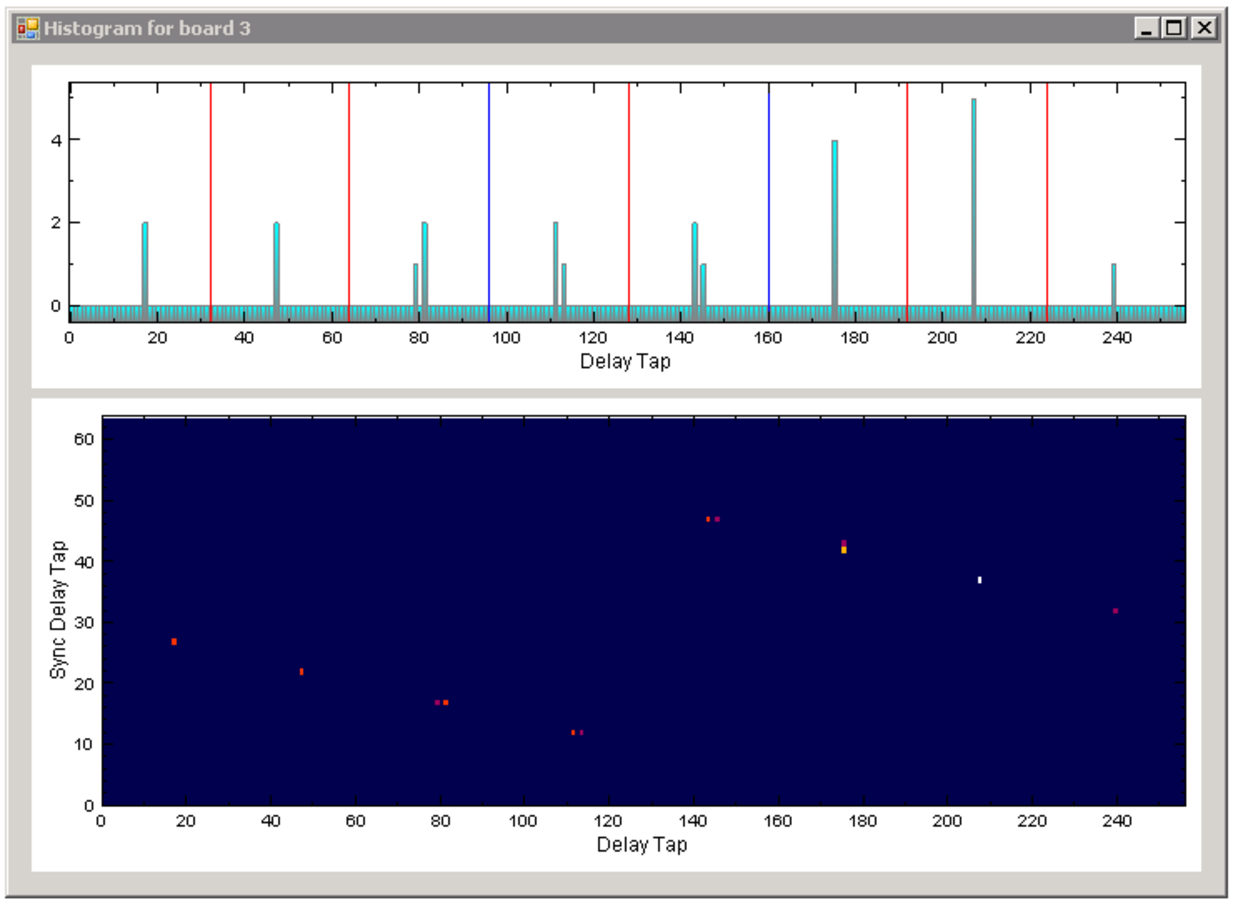
\includegraphics[width=0.6\textwidth]{figures/HistoUncalib.pdf}
				\caption{Histogram for the case the delay value for the board is not set correctly. Please note: the lower panel might differ from board to board, with the ``step'' being at a different position.\label{fig:HistoUncalib}}
			\end{center}
		\end{figure*}
		
		\begin{figure*}[hb]
			\begin{center}
				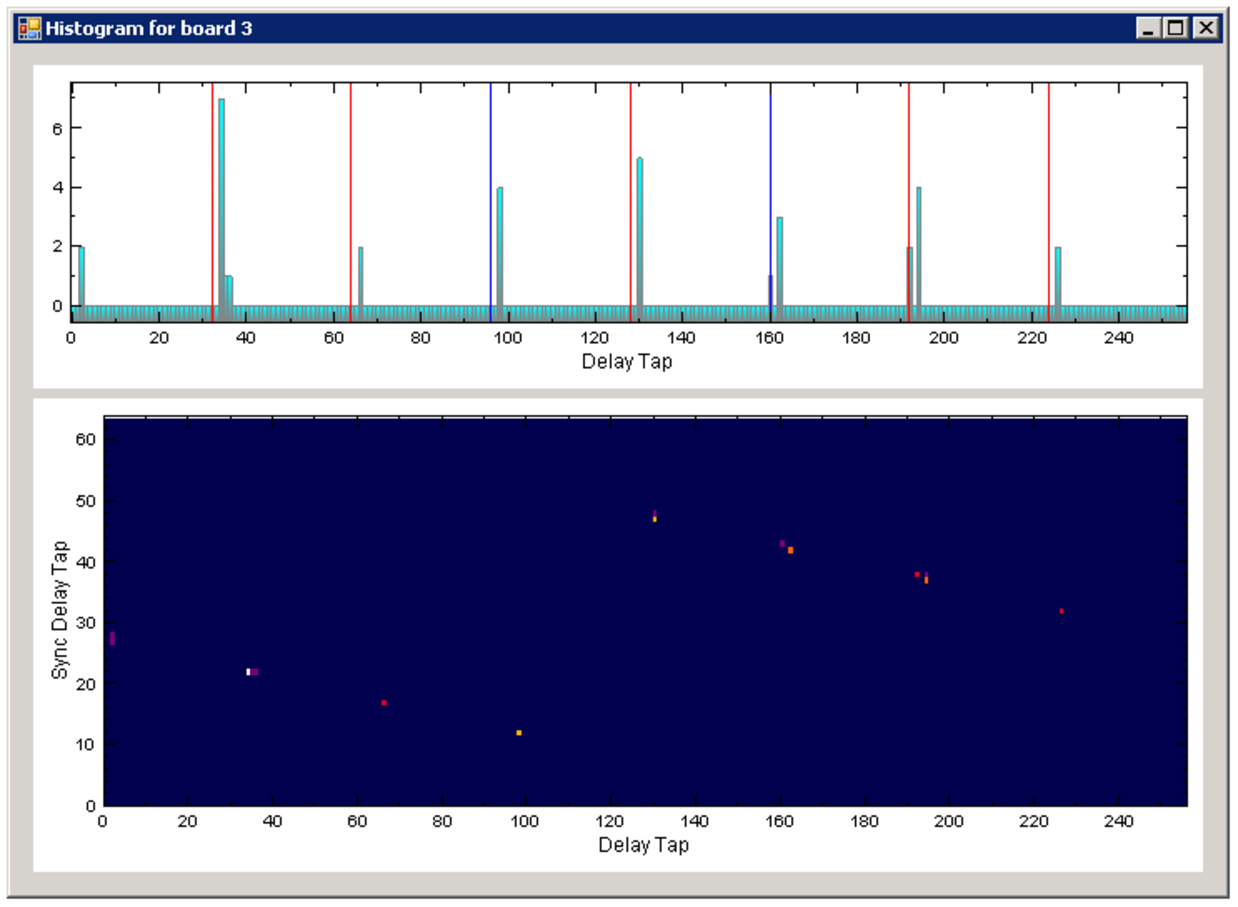
\includegraphics[width=0.6\textwidth]{figures/HistoCalib.pdf}
				\caption{Histogram for the case the delay value for the board is set correctly. Please note: the lower panel might differ from board to board, with the ``step'' being at a different position.\label{fig:HistoCalib}}
			\end{center}
		\end{figure*}
	
	\subsection{Synchronizing a Ndgio5G and an HPTDC8-PCI}
	
		In order to operate a Ndigo5G in sync with one ore more HPTDC8-PCI boards, a board to board interconnection using a Ndigo Extension Board needs to be done. The Ndigo Extension Board has four clock outputs. One of them needs to be connected to the external clock input of the HPTDC using a standard Lemo 00 cable. The Ndigo5G is connected to the Ndigo Extension Board using the Samtec ribbon cable provided with the Ndigo Extension Board. The signals used for synchronization of the boards are transmitted by a standard 10pin ribbon cable connecting the Ndigo Extension Board and the HPTDC. A schematic of all necessary connections is shown in Figure \ref{fig:InterconNdigo}.\par

		In principle the user can use the standard device drivers of the Ndigo5G and the HPTDC8-PCI to perform data acquisition. It is, however, recommended to use the cronoSync-library, which is a part of the cronoTools provided with with the Ndigo5G device driver. CronoSync offers an easy 
group-based access to the data recorded and handles the synchronization of all cronologic data ac-quisition devices used. A detailed description of cronoTools and cronoSync can be found in the cronoTools user guide.

		\begin{figure*}[hb]
			\begin{center}
				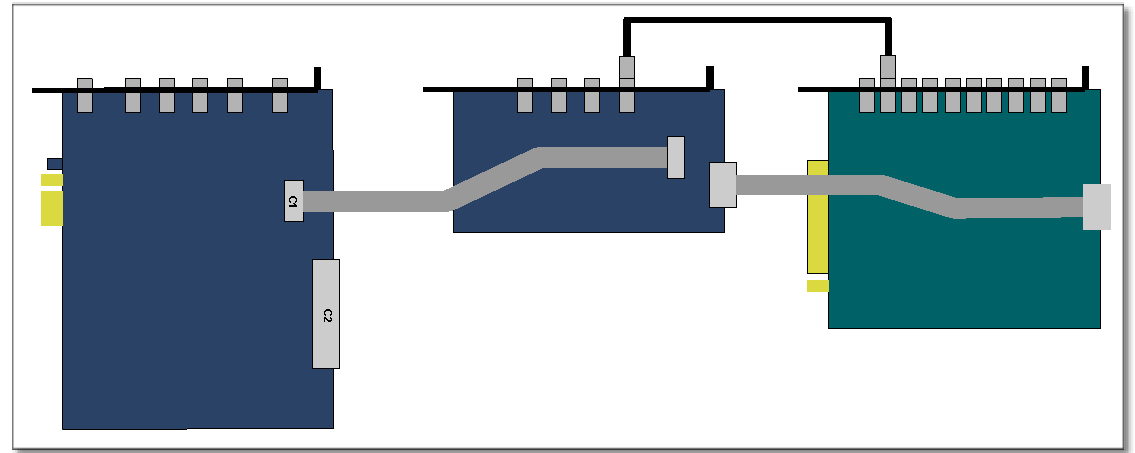
\includegraphics[width=\textwidth]{figures/InterconNdigo.pdf}
				\caption{\label{fig:InterconNdigo} Interconnection scheme of a Ndigo5G (left) and a HPTDC8-PCI (right) using a Ndigo Extension Board (middle).}
			\end{center}
		\end{figure*}
	
	\section{Performing a firmware update}
	
		After installing the Ndigo device driver, a firmware update tool is available. By choosing ``NdigoFirmwareGUI.exe'' a firmware update can be performed. After invoking the application a window as shown in Figure \ref{fig:Firmware} will appear. The tool can be used for updating the firmware and to create a backup of the on-board calibration data of the Ndigo unit. If several boards are present, the one which is going to be used can be selected in the upper left corner of the window. Pressing the ``Backup'' buttons a backup of the firmware or the calibration data will be created, respectively. In order to perform a firmware update, chose the ``.ndigorom''-file to used by pressing ``Browse''. The file contains the firmware PROMs for all boards of the Ndigo product line. By pressing ``Flash'' the firmware is written to the board. ``Verify'' can be used to compare the data stored inside the PROM to the one inside a file.\par
		
		\begin{figure*}[ht]
			\begin{center}
				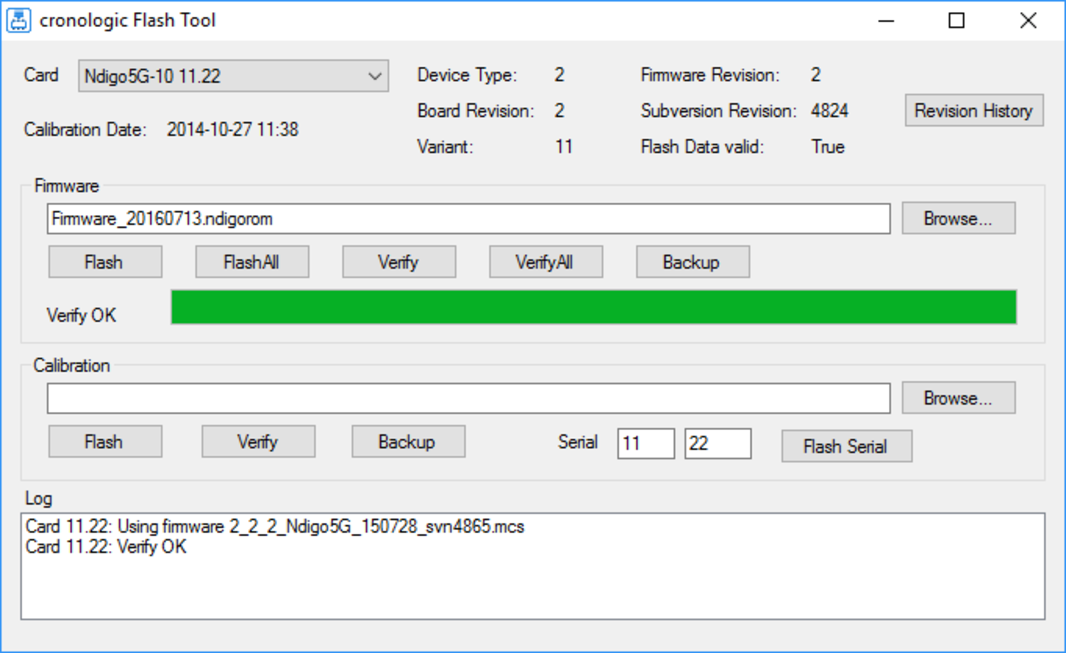
\includegraphics[width=0.8\textwidth]{figures/Firmware.pdf}
				\caption{\label{fig:Firmware}The firmware update and calibration data backup tool as provided with the Ndigo device driver.}
			\end{center}
		\end{figure*}

\textbf{Important note:} The new firmware will only be used after a power cycle, i.e. after switching the PC (or Ndigo crate) off and back on. A simple reboot is not sufficient. Therefore the information shown in the upper half of the application window does not change right after flashing a new firmware.\par
After flashing and shutting the PC or the crate off and on again it is recommended to perform a window calibration. The tool ``WindowCalibration'' is provided for that purpose within the driver installation. The omission of the calibration process leads to longer execution times of applications using that firmware, since the calibration is performed then instead.
	
	\section{Calibrating the TDC}
	
		After each update of the Ndigo5G-10 firmware the TDC has to be calibrated. The calibration is done with the tool ``TDC\tu Calibration.exe'' which is available after installing the Ndigo device driver. After invoking the application a window as shown in Figure \ref{fig:Calib} will appear.\par

		\begin{figure*}[ht]
			\begin{center}
				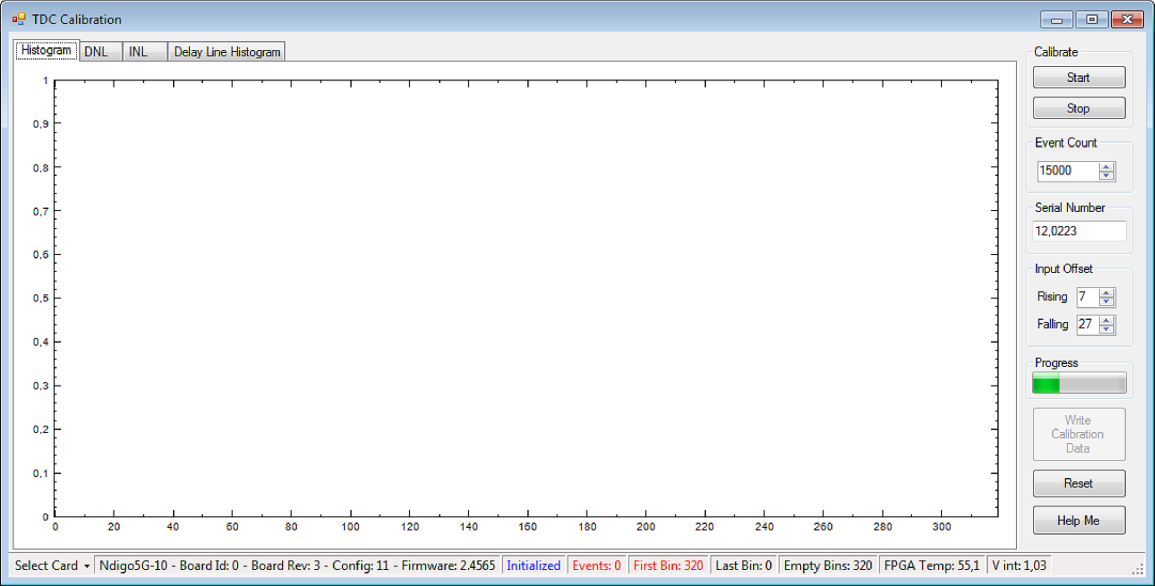
\includegraphics[width=0.8\textwidth]{figures/Calib.pdf}
				\caption{\label{fig:Calib}The TDC calibration tool as provided with the Ndigo device driver.}
			\end{center}
		\end{figure*}
		
		The calibration procedure is as follows:
		
		\begin{enumerate}
			\item Connect an external pulse signal to the Trigger input. The signal should be low active with a frequency in the kHz range. It must not be synchronized to the clock source of the Ndigo5G-10. The input frequency must not exceed 10 MHz. The pulse low and high width has to be at least 10ns each.
			\item Set \textit{Serial Number} according to the sticker on the card if the shown value is not correct.
			\item Start capturing pulse events by pressing the \textit{Start} button.
			\item Adjust the \textit{Input Offset} so that \textit{First Bin} is in the range of 4 to 16. If \textit{First Bin} is less than 4, increment \textit{Input Offset} by one. If \textit{First Bin} is greater than 16 decrement \textit{Input Offset} by one. Repeat increment/decrement until \textit{First Bin} is in the range of 4 to 16. Depending on 
the firmware revision the \textit{Input Offset} value for a successful calibration may be in the range of 6 – 10 or 28 – 32.
			\item When the \textit{Write Calibration Data} button becomes enabled press it to update the calibration data on the card.
			\item Calibration done!
		\end{enumerate}
		
		The card can only be successfully calibrated if:
		
		\begin{itemize}
			\item \textit{First Bin} is in the range of 4 to 16
			\item \textit{Empty Bins} is less than (First Bin + 4)
			\item at least 10,000 events have been captured
			\item a valid serial number is set.
		\end{itemize}
		
		\textbf{Important note:} If the application reports an error check if the input pulse is within specification.
    \chapter{Driver Programming API}
        % SVN Info:
% $Date: 2019-06-04 16:01:22 +0200 (Di, 04 Jun 2019) $
% $Rev: 4980 $
% $Author: andreas $
The API is a DLL with C linkage. The functions provided by the DLL are declared in \textsf{Ndigo\tu interface.h}. \par

\section{Constants}

	\crondef{NDIGO\tu CHANNEL\tu COUNT 4}\\
	The number of analog input channels.\par

	\crondef{NDIGO\tu GATE\tu COUNT 4}\\
	The number of gating blocks.\par

	\crondef{NDIGO\tu TRIGGER\tu COUNT 16}\\
	The number of triggers. Two per analog input, one per digital input plus some specials.\par

	\crondef{NDIGO\tu ADD\tu TRIGGER\tu COUNT 6}\\
	Additional set of triggers for digital inputs.

	\section{Initialization}

		\cronvar{int}{ndigo\tu count\tu devices(}\cronvar{int}{*error\tu code}, \cronvar{char}{**error\tu message)}\\
		Return the number of boards that are supported by this driver in the system.\par

		\cronvar{int}{ndigo\tu get\tu default\tu init\tu parameters(}\cronvar{ndigo\tu init\tu parameters}{*init)}\\
		Get a set of default parameters to feed into \textsf{ndigo\tu init()}. This must always be used to initialize the \textsf{ndigo\tu init\tu parameter structure}.\par

		\cronvar{ndigo\tu device}{*ndigo\tu init(}\cronvar{ndigo\tu init\tu parameters}{*params}, \cronvar{int}{*error\tu code}, \cronvar{char}{**error\tu message)}\\
		Open and initialize the Ndigo board with the given index. With \textsf{error\tu code} and \textsf{error\tu message} the user must provide pointers where to buffers where error information should be written by the driver. The buffer for the error message must by at least 80 chars long.\par
		
		Params is a structure of type \textsf{ndigo\tu init\tu parameters} that must be completely initialized.\par
		
		\cronvar{int}{ndigo\tu close(}\cronvar{ndigo\tu device}{*device)}\\
		Finalize the driver for this device.
	
		\subsection{Structure ndigo\tu init\tu parameters}
		
			\cronvar{int}{version}\\
			Must be set to \textsf{NDIGO\tu API\tu VERSION}\par
			
			\cronvar{int}{card\tu index}\\
			The index in the list of Ndigo5G boards that should be initialized. There might be multiple boards in the system that are handled by this driver as reported by \textsf{ndigo\tu count\tu devices}. This index selects one of them. Boards are enumerated depending on the PCIe slot. The lower the bus number and the lower the slot number the lower the card index.\par

			\cronvar{int}{board\tu id}\\
			This 8 bit number is filled into each packet created by the board and is useful if data streams of multiple boards will be merged. If only Ndigo5G cards are used this number can be set to the card index. If boards of different types that use a compatible data format are used in a system each board should get a unique id. Can be changed with \textsf{int ndigo\tu set\tu board\tu id(ndigo\tu device *device, int board\tu id)}.\par
	
			\cronvar{ndigo\tu bool\tu t}{use\tu external\tu clock}\\
			Use 10MHz clock supplied by IPC flat band cable. Must be set for all slaves.\par
			
			\cronvar{ndigo\tu bool\tu t}{drive\tu external\tu clock}\\
			Drive internal 10MHz clock of this board to IPC flat band cable. Must be set for master.\par

			\cronvar{ndigo\tu bool\tu t}{is\tu slave}\\
			Data acquisition of this board is controlled by the master board.\par

			\cronvar{int}{sync\tu period}\\
			Period of the multicard sync pulse. Should be set to 4 (default) when using several Ndigo boards in sync. Ignored for single board setups. The Ndigo5G has 4 phases relative to the global 10MHz clock.\par
			
			\cronvar{int}{sync\tu delay}\\
			Fine tap delay for incoming sync signals.\par
			
			\cronvar{ndigo\tu bool\tu t}{force\tu window\tu calibration}\\
			If true/1, valid data window is detected at initialization. Default value is false/0: values from flash memory are used in order to set data window to correct position.

			\cronvar{ndigo\tu bool\tu t}{hptdc\tu sync\tu enabled}\\
			A HPTDC is connected to this board. Enables the clock and sync line from the Ndigo5G to the HPTDC.\par

			\cronvar{\tu \tu int64}{buffer\tu size[8]}\\
			The minimum size of the DMA buffer. If set to 0 the default size of 16MByte is used. Ndigo5G only uses \textsf{buffer\tu size[0]}.\par

			\cronvar{int}{buffer\tu type}\\
			Must be set to \textsf{NDIGO\tu BUFFER\tu ALLOCATE}.\par

			\cronvar{\tu \tu int64}{buffer\tu address}\\
			Ignored. Might be used for future buffer types.\par

			\cronvar{int}{variant}\\
			Set to 0. Can be used to activate future device variants such as different base frequencies.\par

			\cronvar{int}{device\tu type}\\
			Initialized by \textsf{ndigo\tu get\tu default\tu init\tu parameters()}. Must be left unchanged.
			
			\begin{description}
				\item[] \crondef{CRONO\tu DEVICE\tu HPTDC 0}
				\item[] \crondef{CRONO\tu DEVICE\tu NDIGO5G 1}
				\item[] \crondef{CRONO\tu DEVICE\tu NDIGO250M 2}
			\end{description}
			
			\cronvar{int}{dma\tu read\tu delay}\\
			Initialized by \textsf{ndigo\tu get\tu default\tu init\tu parameters()}. The write pointer update is delay by this number of 4 ns clock periods to hide race conditions between software and DMA.
	\section{Status Information}
		\subsection{Functions for Information Retrieval}
		
			The driver provides functions to retrieve detailed information on the type of board, its configuration, settings and state. The information is split according to its scope and the computational requirements to query the information from the board.\par
			
			\cronvar{int}{ndigo\tu get\tu driver\tu revision()}\\
			Returns the driver version, same format as ndigo\tu static\tu info::driver\tu revision. This function does not require a
			present Ndigo5G device.

			\cronvar{const char*}{ndigo\tu get\tu driver\tu revision\tu str()}\\
			Returns the driver version including SVN build revision as a string. This function does not require a
			present Ndigo5G device.
			
			\cronvar{int}{ndigo\tu get\tu static\tu info(}\cronvar{ndigo\tu device}{*device},\cronvar{ndigo\tu static\tu info}{*info)}\\
			This structure contains information about the board that does not change during run time.\par

			\cronvar{int}{ndigo\tu get\tu param\tu info(}\cronvar{ndigo\tu device}{*device}, \cronvar{ndigo\tu param\tu info}{*info)}\\
			The structure returned by this call contains information that changes indirectly due to configuration changes.\par

			\cronvar{int}{ndigo\tu get\tu fast\tu info(}\cronvar{ndigo\tu device}{*device}, \cronvar{ndigo\tu fast\tu info}{*info)}\\
			This call returns a structure that contains dynamic information that can be obtained within a few microseconds.\par

			\cronvar{int}{ndigo\tu get\tu slow\tu info(}\cronvar{ndigo\tu device}{*device}, \cronvar{ndigo\tu slow\tu info}{*info)}\\
			The data reported in this structure requires milliseconds to be obtained. The application should only call it in situation where the program flow can cope with an interruption of that magnitude.
		
		\cronvar{const char*}{ndigo\tu get\tu last\tu error\tu message(}\cronvar{ndigo\tu device}{*device)}\\
		\subsection{Structure ndigo\tu static\tu info}
		
			This structure contains information about the board that does not change during run time. It is provided by the function \textsf{ndigo\tu get\tu static\tu info}.\par
			
			\cronvar{int}{size}\\
			The number of bytes occupied by the structure\par

			\cronvar{int}{version}\\
			A version number that is increased when the definition of the structure is changed. The increment can be larger than one to match driver version numbers or similar. Set to 0 for all versions up to first release.\par

			\cronvar{int}{board\tu id}\\
			Index of the board as passed to the constructor or set via \textsf{int ndigo\tu set\tu board\tu id(ndigo\tu device *device, int board\tu id)}.\par
			
			\cronvar{int}{driver\tu revision}\\
			The lower three bytes contain a triple level hierarchy of version numbers, e.g. 0x010103 encodes version 1.1.3.\par

			A change in the first digit generally requires a recompilation of user applications. Change in the second digit denote significant improvements or changes that don't break compatibility and the third digit changes with minor bugfixes and similar updates.\par

			\cronvar{int}{firmware\tu revision}\\
			Firmware revision of the FPGA configuration. This increments only when there is a functional change.\par

			\cronvar{int}{board\tu revision}\\
			0 for experimental prototypes labeled ``Rev. 1''\\
			2 for the version produced until 2010 labeled ``Rev. 2''`\\
			3 for the version produced starting in 2011 labeled ``Rev. 3''\\
			
			\cronvar{int}{board\tu configuration}\\
			Describes the schematic configuration of the board.\par

			\noindent\textit{For board revision 0 this always reads 0.}\par

			\noindent\textit{For board revision 2 the following assignments are valid:}\par

			\noindent If Bit 3 = 0 this following is valid:\\
			Bit 0 determines the ADC resolution. ($0 = 8-\text{bit}$ or $1 = 10-\text{bit}$ ).\\
			Bit 1 determines whether the TDC-oscillator is present ($0 = \text{oscillator present}$, $1 = \text{simple trigger}$).\\
			Bit 2 determines the input connectors ($0 = \text{single ended}$, $1 = \text{differential}$).\par

			\noindent Bit $3 = 1$ signifies a special version of the board\\
			0xA is Ndigo1250M-12 single ended with digital trigger\\
			0x8 is Ndigo5G-8 single ended with digital trigger\par
			
			\noindent\textbf{For Board revision 3 the following assignments are valid:}\par

			\noindent Bit 2 determines the input connectors ($0 = \text{single ended}$, $1 = \text{differential}$).\par

			\noindent The other bits have one of the following patterns [Bits 3...0]\par

			\noindent 0010 Ndigo5G-10 2.5u 10\\
			0011 Ndigo5G-8-AQ 2.5u 8\\
			0110 Ndigo5G-10-Diff 560pF 10 DIFF\\
			1000 Ndigo5G-8 560pF 8+\\
			1010 Ndigo1250M-12 2.2uF 12 Sciex DC\\
			1011 Ndigo5G-10 560pF 10\\
			1110 Ndigo5G-Sciex 2.2uF 10 Sciex Infiniband, DIFF\\
			1111 Ndigo5G-Roent = fADC4/10 560pF 10\par

			\cronvar{int}{adc\tu resolution}\\
			Number of bits of the ADC, set to 0 if unknown.\par

			\cronvar{double}{nominal\tu sample\tu rate}\\
			Sample rate in once channel mode. Usually $5.0e9 = 5 Gsps$.\par

			\cronvar{double}{analog\tu bandwidth}\\
			9.5e8 for \SI{950}{\MHz}.
			
			\cronvar{int}{chip\tu id}\\
			16 bit factory ID of the ADC chip\par
			
			\cronvar{int}{board\tu serial}\\
			Serial number with the year minus 2000 in the highest 8 bits of the integer and a running number in the lower 24 bits. This number is identical with the one on the label on the board.\par

			\cronvar{int}{flash\tu serial\tu low}\\
			\cronvar{int}{flash\tu serial\tu high}\\
			64 bit manufacturer serial number of the flash chip.\par

			\cronvar{int}{flash\tu valid}\\
			If not 0 the driver found valid calibration data in the flash on the board and is using it.\par

			\cronvar{ndigo\tu bool\tu t}{dc\tu coupled}\\
			Returns false for the standard AC coupled Ndigo5G.\par

			\cronvar{int}{subversion\tu revision}\\
			A number to track builds of the firmware in more detail than the firmware revision. It changes with every change in the firmware, even if there is no visible effect for the user.\par
			
			\cronvar{char}{calibration\tu date[20]}\\
			DIN EN ISO 8601 string YYYY-MM-DD HH:DD describing the time when the card was calibrated.
		
		\subsection{Structure ndigo\tu param\tu info}
		
			\cronvar{int}{size}\\
			The number of bytes occupied by the structure.\par

			\cronvar{int}{version}\\
			A version number that is increased when the definition of the structure is changed. The increment can be larger than one to match driver version numbers or similar. Set to 0 for all versions up to
first release.\par

			\cronvar{double}{bandwidth}\\
			Bandwidth setting of the ADC. Note: This is not the bandwidth of the analog board frontend. \par

			\cronvar{double}{sample\tu rate}\\
			Sample rate. This is 1.25e9, 2.5e9 or 5.0e9 depending on the current ADC mode. $\text{sample\tu rate}\cdot \text{channels} = 5.0e9$.\par
			
			\cronvar{double}{sample\tu period}\\
			The period one sample in the data represents in picoseconds\par

			\cronvar{int}{board\tu id}\\
			The number the board uses to identify the data source in the output data stream.\par

			\cronvar{int}{channels}\\
			Number of channels. 1, 2 or 4 depending on the ADC mode chosen. $\text{sample\tu rate}\cdot\text{channels} = 5.0e9$.\par

			\cronvar{int}{channel\tu mask}\\
			Mask with a set bit for each enabled input channel.\par

			\cronvar{\tu\tu int64}{total\tu buffer}\\
			The total amount of the DMA buffer in bytes.\par

%			\cronvar{\tu\tu int64}{free\tu buffer}\\
%			Unused portion of the DMA buffer in bytes.\par
		
		\subsection{Structure ndigo\tu fast\tu info}
		
			\cronvar{int}{size}\\
			The number of bytes occupied by the structure\par

			\cronvar{int}{version}\\
			A version number that is increased when the definition of the structure is changed. The increment can be larger than one to match driver version numbers or similar. Set to 0 for all versions up to first release.\par

			\cronvar{int}{adc\tu rpm}\\
			Speed of the ADC fan. Reports 0 if no fan is present.\par

			\cronvar{int}{fpga\tu rpm}\\
			Speed of the FPGA fan. Reports 0 if no fan is present.\par

			\cronvar{int}{alerts}\\
			Alert bits from the system monitor.\par
			
			\noindent Bit 0 : FPGA temperature alert ($> 85^{\circ}C$)\\
			Bit 1 : Internal FPGA voltage out of range ($< 1.01V$ or $> 1.08V$)\\
			Bit 2 : FPGA auxiliary voltage out of range. ($< 2.375V$ or $>  2.625V$)\\
			Bit 3 : FPGA temperature critical ($> 125^{\circ}C$)\\
			Bit 4 : ADC temperature alert ($> 90^{\circ}C$)\\
			Bit 5 : ADC temperature critical ($> 100^{\circ}C$): will automatically be turned off.\par

			\cronvar{double}{voltage\tu aux}\\
			Auxiliary FPGA voltage, nominal 2.5V\par

			\cronvar{double}{voltage\tu int}\\
			Internal FPGA voltage, nominal 1.0V\par

			\cronvar{double}{fpga\tu temperature}\\
			In $^\circ$C measured on die.\par

			\cronvar{int}{pcie\tu link\tu width}\\
			Number of PCIe lanes that the card uses. Should be 4 for Ndigo5G. \par %% and 8 for Ndigo5G-Sciex.\par

			\cronvar{int}{pcie\tu max\tu payload}\\
			Maximum size in bytes for one PCIe transaction, depends on system configuration.\par
		
		\subsection{Structure ndigo\tu slow\tu info}
		
			\cronvar{int}{size}\\
			The number of bytes occupied by the structure.\par

			\cronvar{int}{version}\\
			A version number that is increased when the definition of the structure is changed. The increment can be larger than one to match driver version numbers or similar. Set to 0 for all versions up to
first release.\par

			\cronvar{double}{adc\tu temperature}\\
			ADC temperature in $^{\circ}C$ measured on die.\par

			\cronvar{double}{board\tu temperature}\\
			In $^{\circ}C$.
		
	\section{Configuration}
	
		The device is configured with a configuration structure. The user should first obtain a structure that contains the default settings of the device read from an on board ROM , than modify the structure as needed for the user application and use the result to configure the device.\par

		\cronvar{int}{ndigo\tu get\tu default\tu configuration(}\cronvar{ndigo\tu device}{*device,} \cronvar{ndigo\tu configuration}{*config)}\par

		\cronvar{int}{ndigo\tu get\tu current\tu configuration(}\cronvar{ndigo\tu device}{*device,} \cronvar{ndigo\tu configuration}{*config)}\par
		
		\cronvar{int}{ndigo\tu configure(}\cronvar{ndigo\tu device} {*device,} \cronvar{ndigo\tu configuration}{*config)}\par

		\cronvar{int}{ndigo\tu set\tu board\tu id(}\cronvar{ndigo\tu device}{*device,} \cronvar{int}{board\tu id)}\\
		The \textsf{board\tu id} can be changed after initialization of the card. If cronotools are used the \textsf{board\tu id} changes have to be done before cronotools initialization.	
	
		\subsection{Structure ndigo\tu configuration}
		
			This is the structure containing the configuration information. It is used in conjunction with \textsf{ndigo\tu get\tu default\tu configuration}, \textsf{ndigo\tu get\tu current\tu configuration} and \textsf{ndigo\tu configure}.\par

			It uses internally the structures \textsf{ndigo\tu trigger\tu block} and \textsf{ndigo\tu trigger}.\par

			\cronvar{int}{size}\\
			The number of bytes occupied by the structure.\par

			\cronvar{int}{version}\\
			A version number that is increased when the definition of the structure is changed. The increment can be larger than one to match driver version numbers or similar. Set to 0 for all versions up to first release.\par

			\cronvar{int}{reserved1}\\
			Reserved for internal usage. Do not change.\par

			\cronvar{int}{adc\tu mode}\\
			Constant describing the ADC mode\par

			\crondef{NDIGO\tu ADC\tu MODE\tu ABCD 0}\\
			\crondef{NDIGO\tu ADC\tu MODE\tu AC 4}\\
			\crondef{NDIGO\tu ADC\tu MODE\tu BC 5}\\
			\crondef{NDIGO\tu ADC\tu MODE\tu AD 6}\\
			\crondef{NDIGO\tu ADC\tu MODE\tu BD 7}\\
			\crondef{NDIGO\tu ADC\tu MODE\tu A 8}\\
			\crondef{NDIGO\tu ADC\tu MODE\tu B 9}\\
			\crondef{NDIGO\tu ADC\tu MODE\tu C 10}\\
			\crondef{NDIGO\tu ADC\tu MODE\tu D 11}\\
			\crondef{NDIGO\tu ADC\tu MODE\tu AAAA 12}\\
			\crondef{NDIGO\tu ADC\tu MODE\tu BBBB 13}\\
			\crondef{NDIGO\tu ADC\tu MODE\tu CCCC 14}\\
			\crondef{NDIGO\tu ADC\tu MODE\tu DDDD 15}\\
			\crondef{NDIGO\tu ADC\tu MODE\tu A12 28} // not available on all boards\\
			\crondef{NDIGO\tu ADC\tu MODE\tu B12 29} // not available on all boards\\
			\crondef{NDIGO\tu ADC\tu MODE\tu C12 3}0 // not available on all boards\\
			\crondef{NDIGO\tu ADC\tu MODE\tu D12 31} // not available on all boards\par

			\cronvar{double}{bandwidth}\\
			Set to the minimum bandwidth required for the application. Lower bandwidth results in reduced noise. The driver will set the ADC to the minimum setting that has at least the desired bandwidth and report the selected bandwidth in the \textsf{ndigo\tu param\tu info} structure. The -8, -10 and -12 versions currently supports 1GHz and 3GHz bandwidth, the -8AQ version supports 2GHz, 1.5GHz, 600MHz and 500 MHz. The bandwidth of the analog frontend of the board remains unchanged at about \SI{950}{\MHz}.
			\par

			\cronvar{ndigo\tu bool\tu t}{reserved}\\
			\cronvar{ndigo\tu bool\tu t}{tdc\tu enabled}\\
			Enable capturing of TDC measurements on external digital input channel.\par
			
			\cronvar{ndigo\tu bool\tu t}{tdc\tu fb\tu enabled}\\
			Enable enhanced TDC resolution. Currently not implemented.\par

			\cronvar{double}{analog\tu offset[NDIGO\tu CHANNEL\tu COUNT]}\\
			Sets the input DC offset-values to +- this value in volts. Defaults to 0.\par

			\cronvar{double}{dc\tu offset[2]}\\
			Sets the DC offset in volts for the TDC trigger input (index 1) and the GATE input (index 0). The default is -0.35 which is a good setting vor \SI{0.8}{\volt} negative NIM pulses.
			The values are limited by the driver to the range [-1.25, 1.25]. When using the TDC, nonnegative values for index 1 throw an error. \par

			\cronvar{ndigo\tu trigger}{trigger[NDIGO\tu TRIGGER\tu COUNT + NDIGO\tu ADD\tu TRIGGER\tu COUNT]}\\
			Configuration of the external trigger sources. Threshold is ignored for entries 8 and above.\par
			
			The trigger indexes refer to the entry in the trigger array and are defined like this:\par

			\crondef{NDIGO\tu TRIGGER\tu A0 0}\\
			\crondef{NDIGO\tu TRIGGER\tu A1 1}\\
			\crondef{NDIGO\tu TRIGGER\tu B0 2}\\
			\crondef{NDIGO\tu TRIGGER\tu B1 3}\\
			\crondef{NDIGO\tu TRIGGER\tu C0 4}\\
			\crondef{NDIGO\tu TRIGGER\tu C1 5}\\
			\crondef{NDIGO\tu TRIGGER\tu D0 6}\\
			\crondef{NDIGO\tu TRIGGER\tu D1 7}\\
			\crondef{NDIGO\tu TRIGGER\tu TRIGGER 8}\\
			\crondef{NDIGO\tu TRIGGER\tu TDC 8}\\
			\crondef{NDIGO\tu TRIGGER\tu GATE 9}\\
			\crondef{NDIGO\tu TRIGGER\tu BUS0 10}\\
			\crondef{NDIGO\tu TRIGGER\tu BUS1 11}\\
			\crondef{NDIGO\tu TRIGGER\tu BUS2 12}\\
			\crondef{NDIGO\tu TRIGGER\tu BUS3 13}\par
			
			\crondef{NDIGO\tu TRIGGER\tu AUTO 14}\\
			\crondef{NDIGO\tu TRIGGER\tu ONE 15}\par
			
			Always positive edge-sensitive sources:\\
			\crondef{NDIGO\tu TRIGGER\tu TDC\tu PE 16}\\
			\crondef{NDIGO\tu TRIGGER\tu GATE\tu PE 17}\\
			\crondef{NDIGO\tu TRIGGER\tu BUS0\tu PE 18}\\
			\crondef{NDIGO\tu TRIGGER\tu BUS1\tu PE 19}\\
			\crondef{NDIGO\tu TRIGGER\tu BUS2\tu PE 20}\\
			\crondef{NDIGO\tu TRIGGER\tu BUS3\tu PE 21}\par

			\cronvar{ndigo\tu trigger\tu block}{trigger\tu block[NDIGO\tu CHANNEL\tu COUNT + 1]}\\
			A structure describing the trigger settings of the four channels plus the timestamp channel. In some modes not all channels are used.\par

			\cronvar{ndigo\tu gating\tu block}{gating\tu block[4]}\\
			A structure describing the gating blocks that can be used by the trigger blocks to filter triggers.\par

			\cronvar{ndigo\tu extension\tu block}{extension\tu block[NDIGO\tu EXTENSION\tu COUNT]}\\
			A structure describing the routing of the 4 digital channels of the Ndigo extension board to the trigger matrix.\par

			\cronvar{int}{drive\tu bus[4]}\\
			Enable output drive for each of the four external sync lines. Each integer represents a bitmask selecting the trigger sources for that line. The bit mapping is described in section ``Structure \textsf{ndigo\tu trigger\tu block}'' on page \pageref{cp:triggerblock}.\par

			\cronvar{int}{auto\tu trigger\tu period}\\
			\cronvar{int}{auto\tu trigger\tu random\tu exponent}\\
			Create a trigger either periodically or randomly. There are two parameters $M = \text{trigger\tu period}$ and $N = \text{random\tu exponent}$ that result in a distance between triggers of
			
			\begin{align}
				T = 1 + M + [1...2^N]
			\end{align}

			clock cycles.
			
			\begin{align}
				0 \leq M < 2^{32}\\
				0 \leq N < 32
			\end{align}					
		
			There is no enable or reset as the usage of this trigger can be configured in the trigger block channel source field.\par

			\cronvar{int}{output\tu mode}\\
			Defines the data representation in the output. Signed16 scales and INL-corrects the input. RAW directly presents the ADC values.\par
			
			\crondef{NDIGO\tu OUTPUT\tu MODE\tu SIGNED16 0}\\
			\crondef{NDIGO\tu OUTPUT\tu MODE\tu RAW 1}\\
			\crondef{NDIGO\tu OUTPUT\tu MODE\tu CUSTOM 2}\\
			\crondef{NDIGO\tu OUTPUT\tu MODE\tu CUSTOM\tu INL 3}\par
			
			\cronvar{lut\tu func}{custom\tu lut}\\
			If the \textsf{output\tu mode} is set to \textsf{NDIGO\tu OUTPUT\tu MODE\tu CUSTOM} or\\\textsf{NDIGO\tu OUTPUT\tu MODE\tu CUSTOM\tu INL} this function is used for mapping from ADC value to output value. The driver will call this function with a value from -1 to +1 and the function must return the corresponding signed 16 bit value that the board should return for an input voltage relative to the full scale range.\par

			\cronvar{typedef short}{(*lut\tu func)(}\cronvar{int}{channel,} \cronvar{float}{x)}\par

			This can be used e.g. for custom INL, offset and gain correction that covers user front end electronics. It can also invert the signal or correct the effect of logarithmic input amplifiers etc.\par
			
			The LUT is applied on the board, thus using it does not cause any additional CPU load. In the mode ``\textsf{NDIGO\tu OUTPUT\tu MODE\tu CUSTOM\tu INL}'' the on-board INL correction table is applied before the user function, while ``\textsf{NDIGO\tu OUTPUT\tu MODE\tu CUSTOM}'' does not perform INL correction. In order to use the user lookup table functionality \textsf{lut\tu func} must be set to a pointer to the LUT-function.
		
		\subsection{Structure ndigo\tu trigger}
		
			\cronvar{short}{threshold}\\
			Sets the threshold for the trigger block within the range of the ADC data of -32768 and +32768.\par

			For trigger indices \textsf{NDIGO\tu TRIGGER\tu TDC} to \textsf{NDIGO\tu TRIGGER\tu BUS3\tu PE} the threshold is ignored.\par

			\cronvar{ndigo\tu bool\tu t}{edge}\\
			If set this trigger implements edge trigger functionality else this is a level trigger.\par

			For trigger indices \textsf{NDIGO\tu TRIGGER\tu AUTO} and \textsf{NDIGO\tu TRIGGER\tu ONE} this is ignored.\par
			
			For trigger indices \textsf{NDIGO\tu TRIGGER\tu TDC\tu PE} to \textsf{NDIGO\tu TRIGGER\tu BUS3\tu PE} this must be set.\par
	
			\cronvar{ndigo\tu bool\tu t}{rising}\\
			If set trigger on rising edges or when above threshold.\par

			For trigger indices \textsf{NDIGO\tu TRIGGER\tu AUTO} and \textsf{NDIGO\tu TRIGGER\tu ONE} this is ignored.\par

			For trigger indices \textsf{NDIGO\tu TRIGGER\tu TDC\tu PE} to \textsf{NDIGO\tu TRIGGER\tu BUS3\tu PE} this must be set.
		
		\subsection{Structure ndigo\tu trigger\tu block\label{cp:triggerblock}}
		
		\cronvar{ndigo\tu bool\tu t}{enabled}\\
		Activate triggers on this channel.\par

		\cronvar{ndigo\tu bool\tu t}{retrigger}\\
		If a new trigger condition occurs while the postcursor is acquired the packet is extended by starting a new postcursor. Otherwise the new trigger is ignored and the packet ends after the precursor of the first trigger.\par

		The retrigger setting is ignored for the timestamp channel.\par

		\cronvar{ndigo\tu bool\tu t}{reserved1}\\
		Defaults to false. Do not change.\par

		\cronvar{ndigo\tu bool\tu t}{reserved2}\\
		Defaults to false. Do not change.\par

		\cronvar{int}{precursor}\\
		Precursor in multiples of 3.2ns. The amount of data preceding a trigger that is captured.\par
		
		The precursor setting is ignored for the timestamp channel.\par

		\cronvar{int}{length}\\
		In multiples of 3.2ns.\par

		The total amount of data that is recorded in addition to the trigger window. Precursor determines how many of these are ahead of the trigger and how many are appended after the trigger. In edge trigger mode the trigger window always is 3.2ns wide, in level trigger mode it is as long as the
trigger condition is fulfilled.\par

		The length setting is ignored for the timestamp channel.\par

		\cronvar{int}{sources}\\
		A bit mask with a bit set for all trigger sources that can trigger this channel.\par
		
		\begin{tabular}{lc}
			\crondef{NDIGO\tu TRIGGER\tu SOURCE\tu A0} & 0x00000001\\
			\crondef{NDIGO\tu TRIGGER\tu SOURCE\tu A1} & 0x00000002\\
			\crondef{NDIGO\tu TRIGGER\tu SOURCE\tu B0} & 0x00000004\\
			\crondef{NDIGO\tu TRIGGER\tu SOURCE\tu B1} & 0x00000008\\
			\crondef{NDIGO\tu TRIGGER\tu SOURCE\tu C0} & 0x00000010\\
			\crondef{NDIGO\tu TRIGGER\tu SOURCE\tu C1} & 0x00000020\\
			\crondef{NDIGO\tu TRIGGER\tu SOURCE\tu D0} & 0x00000040\\
			\crondef{NDIGO\tu TRIGGER\tu SOURCE\tu D1} & 0x00000080\\
			\crondef{NDIGO\tu TRIGGER\tu SOURCE\tu TDC} & 0x00000100\\
			\crondef{NDIGO\tu TRIGGER\tu SOURCE\tu GATE} & 0x00000200\\
			\crondef{NDIGO\tu TRIGGER\tu SOURCE\tu BUS0} & 0x00000400\\
			\crondef{NDIGO\tu TRIGGER\tu SOURCE\tu BUS1} & 0x00000800\\
		\end{tabular}\\
		\begin{tabular}{lc}
			\crondef{NDIGO\tu TRIGGER\tu SOURCE\tu BUS2} & 0x00001000\\
			\crondef{NDIGO\tu TRIGGER\tu SOURCE\tu BUS3} & 0x00002000
		\end{tabular}\\
		\begin{tabular}{lc}
			\crondef{NDIGO\tu TRIGGER\tu SOURCE\tu AUTO} & 0x00004000\\
			\crondef{NDIGO\tu TRIGGER\tu SOURCE\tu ONE} & 0x00008000
		\end{tabular}\\
		\begin{tabular}{lc}
			\crondef{NDIGO\tu TRIGGER\tu SOURCE\tu TDC\tu PE} & 0x01000000\\
			\crondef{NDIGO\tu TRIGGER\tu SOURCE\tu GATE\tu PE} & 0x02000000\\
			\crondef{NDIGO\tu TRIGGER\tu SOURCE\tu BUS0\tu PE} & 0x04000000\\
			\crondef{NDIGO\tu TRIGGER\tu SOURCE\tu BUS1\tu PE} & 0x08000000\\
			\crondef{NDIGO\tu TRIGGER\tu SOURCE\tu BUS2\tu PE} & 0x10000000\\
			\crondef{NDIGO\tu TRIGGER\tu SOURCE\tu BUS3\tu PE} & 0x20000000
		\end{tabular}
		
		\cronvar{int}{gates}\par
		
		\begin{tabular}{lc}
			\crondef{NDIGO\tu TRIGGER\tu GATE\tu NONE} & 0x0000\\
			\crondef{NDIGO\tu TRIGGER\tu GATE\tu 0}  & 0x0001\\
			\crondef{NDIGO\tu TRIGGER\tu GATE\tu 1}  & 0x0002\\
			\crondef{NDIGO\tu TRIGGER\tu GATE\tu 2}  & 0x0004\\
			\crondef{NDIGO\tu TRIGGER\tu GATE\tu 3}  & 0x0008
		\end{tabular}
		
		\cronvar{double}{minimum\tu free\tu packets;}\\
		This parameter sets how many packets are supposed to fit into the on-board FIFO before a new packet is recorded after the FIFO was full, i.e. a certain amount of free space in the FIFO is demanded before a new packet is written after the FIFO was full. As a measure for the packet length the gatelength set by the user is used. The on-board algorithm checks the free FIFO space only in case the FIFO is full. Therefore, if this number is 1.0 or more at least every second packet in the DMA buffer is guaranteed to have the full length set by the gatelength parameters. In many cases smaller values will also result in full length packets. But below a certain value multiple packets that are cut off at the end will show up.
		
		\subsection{Structure ndigo\tu gating\tu block\label{cp:gatingblock}}
		
			\cronvar{ndigo\tu bool\tu t}{negate}\\
			Invert output polarity. Defaults to false.\par

			\cronvar{ndigo\tu bool\tu t}{retrigger}\\
			Defaults to false. If retriggering is enabled the timer is reset to the value of the start parameter whenever the input signal is set while waiting to reach the stop time.\par

			\cronvar{ndigo\tu bool\tu t}{extend}\\
			Defaults to true. If set, a gate is created with the set timing from the first occurrence of the input trigger even for short gates. If not set, the input signal must persist for the gate to be created. This feature is NOT YET IMPLEMENTED.\par

			\cronvar{ndigo\tu bool\tu t}{reserved1}\\
			Defaults to false. Do not change.\par

			\cronvar{int}{start}\\
			In multiples of 3.2ns. The time from the first input signal seen in the idle state until the gating output is set. The value of start needs to be less or equal to the stop value. Maximum value for start and stop is $2^{16}-1$.\par

			\cronvar{int}{stop}\\
			In multiples of 3.2ns. Maximum allowed value is $2^{16}-1$.\par

			The time from leaving the idle state until the gating output is reset. If retriggering is enabled the timer is reset to the value of the start parameter whenever the input signal is set while waiting to reach the stop time.\par

			\cronvar{int}{sources}\\
			A bit mask with a bit set for all trigger sources that can trigger this channel. The gates cannot use the additional digital trigger sources \textsf{NDIGO\tu TRIGGER\tu SOURCE\tu TDC\tu PE} to\\ \textsf{NDIGO\tu TRIGGER\tu SOURCE\tu BUS3\tu PE}.\par

			\begin{tabular}{lc}
				\crondef{NDIGO\tu TRIGGER\tu SOURCE\tu A0} & 0x00000001\\
				\crondef{NDIGO\tu TRIGGER\tu SOURCE\tu A1} & 0x00000002\\
				\crondef{NDIGO\tu TRIGGER\tu SOURCE\tu B0} & 0x00000004\\
				\crondef{NDIGO\tu TRIGGER\tu SOURCE\tu B1} & 0x00000008\\
				\crondef{NDIGO\tu TRIGGER\tu SOURCE\tu C0} & 0x00000010\\
				\crondef{NDIGO\tu TRIGGER\tu SOURCE\tu C1} & 0x00000020\\
				\crondef{NDIGO\tu TRIGGER\tu SOURCE\tu D0} & 0x00000040\\
				\crondef{NDIGO\tu TRIGGER\tu SOURCE\tu D1} & 0x00000080\\
				\crondef{NDIGO\tu TRIGGER\tu SOURCE\tu TDC} & 0x00000100\\
				\crondef{NDIGO\tu TRIGGER\tu SOURCE\tu GATE} & 0x00000200\\
				\crondef{NDIGO\tu TRIGGER\tu SOURCE\tu BUS0} & 0x00000400\\
				\crondef{NDIGO\tu TRIGGER\tu SOURCE\tu BUS1} & 0x00000800\\
				\crondef{NDIGO\tu TRIGGER\tu SOURCE\tu BUS2} & 0x00001000\\
				\crondef{NDIGO\tu TRIGGER\tu SOURCE\tu BUS3} & 0x00002000\\
				\crondef{NDIGO\tu TRIGGER\tu SOURCE\tu AUTO} & 0x00004000\\
				\crondef{NDIGO\tu TRIGGER\tu SOURCE\tu ONE} & 0x00008000
			\end{tabular}
			
		\subsection{Structure ndigo\tu extension\tu block}
			This structure configures how the inputs from the optional extension board and signals from the synchronization bus are merged.\par

			\cronvar{ndigo\tu bool\tu t}{enable}\\
			Enable routing of digital signal from Ndigo extension board to the according BUSx trigger unit.\par

			\cronvar{ndigo\tu bool\tu t}{ignore\tu cable}\\
			If \textit{false} input signal and BUS signal are ORed before routing to the according BUSx trigger unit. Otherwise only the signal from Ndigo extension board is used.
			
		\subsection{Run Time Control}
		
			\cronvar{int}{ndigo\tu start\tu capture(}\cronvar{ndigo\tu device}{*device)}\par
		
			\cronvar{int}{ndigo\tu pause\tu capture(}\cronvar{ndigo\tu device}{*device)}\par

			\cronvar{int}{ndigo\tu continue\tu capture(}\cronvar{ndigo\tu device}{*device)}\\
			Call this to resume data acquisition after a call to \textsf{ndigo\tu pause\tu capture}.\par

			\cronvar{int}{ndigo\tu stop\tu capture(}\cronvar{ndigo\tu device}{*device)}
		
	\section{Readout\label{cp:readout}}
	
		\cronvar{int}{ndigo\tu read(}\cronvar{ndigo\tu device}{*device,} \cronvar{ndigo\tu read\tu in}{*in,} \cronvar{ndigo\tu read\tu out}{*out)}\\
		Return a pointer to an array of captured data in \textsf{read\tu out}. The result can contain any number of packets of type \textsf{ndigo\tu packet}. \textsf{read\tu in} provides parameters to the driver. A call to this method automatically allows the driver to reuse the memory returned in the previous call.\par

Returns an error code as defined in the structure \textsf{ndigo\tu read\tu out}.\par

		\cronvar{int}{ndigo\tu acknowledge(}\cronvar{ndigo\tu device}{*device,} \cronvar{ndigo\tu packet}{*packet)}\\
		Acknowledge all data up to the packet provided as parameter. This is mandatory if \textsf{acknowledge\tu last\tu read} in the \textsf{ndigo\tu read\tu in} structure is set to false for calls to \textsf{ndigo\tu read}.\par

		This feature allows to either free up partial DMA space early if there will be no call to \textsf{ndigo\tu read} anytime soon. It also allows to keep data over multiple calls to \textsf{ndigo\tu read} to avoid unnecessary copying of data.\par

		\cronvar{int}{ndigo\tu process\tu tdc\tu packet(}\cronvar{ndigo\tu device}{*device,} \cronvar{ndigo\tu packet}{*packet)}\\
		Call on a TDC packet to update the timestamp of the packet with a more accurate value. If called more than once on a packet the timestamp will be invalid.	
	
		\subsection{Input Structure ndigo\tu read\tu in}
		
			\cronvar{ndigo\tu bool\tu t}{acknowledge\tu last\tu read}\\
			If set \textsf{ndigo\tu read} automatically acknowledges packets from the last read.
		
		\subsection{Input Structure ndigo\tu read\tu out}
		
			\cronvar{ndigo\tu packet}{*first\tu packet}\\
			Pointer to the first packet that was capture by the call of \textsf{ndigo\tu read}.\par

			\cronvar{ndigo\tu packet}{*last\tu packet}\\
			Address of header of the last packet in the buffer.\par

			\cronvar{int}{error\tu code}\\
			\crondef{NDIGO\tu READ\tu OK 0}\\
			\crondef{NDIGO\tu READ\tu NO\tu DATA 1}\\
			\crondef{NDIGO\tu READ\tu INTERNAL\tu ERROR 2}\par
			
			\cronvar{const char}{*error\tu message}
		
	\section{Other Functions}
		\subsection{LED control}
		
			There are six LEDs on the front panel. The intensity of the red and green part can be set from 0 to 255. There is no blue component in the current version. Per default all LEDs are set to auto mode. This means that used channels are lit green, activity is shown as yellow on overflow is shown as red.\par

			\cronvar{int}{ndigo\tu set\tu led\tu color(}\cronvar{ndigo\tu device}{*device,} \cronvar{int}{led,} \cronvar{unsigned short}{r,} \cronvar{unsigned short}{g,} \cronvar{unsigned short}{b)}\\
			Set the LED to the selected color. No automatic updates are performed.\par
			
			\cronvar{int}{ndigo\tu set\tu led\tu automode(}\cronvar{ndigo\tu device}{*device,} \cronvar{int}{led)}\\
			Let the selected LED be controlled by hardware. 
    \chapter{Packet Format\label{cp:packetformat}}
        % SVN Info:
% $Date: 2019-06-04 12:35:07 +0200 (Di, 04 Jun 2019) $
% $Rev: 4976 $
% $Author: andreas $
\section{Memory Management}

The \textit{host buffer} is memory on the host's system in which the data recorded by the Ndigo5G is stored until it is acknowledged by the user.

The host buffer is managed by the DMA (direct memory access) driver. The DMA driver can only ever write to the host buffer if enough memory is free. That means, new packets will never overwrite old packets, unless they have been acknowledged.

If the host buffer is full, data may be lost. Then, the \texttt{CRONO\_PACKET\_FLAG\_HOST\_BUFFER\_FULL} bit of \texttt{crono\_packet::flags} is set. To ensure that this does not happen, the user must acknowledge packets fast enough by the analysis software. Note that data only has been lost due to a full host buffer if the \texttt{CRONO\_PACKET\_FLAG\_TRIGGER\_MISSED} bit of \texttt{crono\_packet::flags} is set.

\subsection{Acknowledge Packets}
A packet in the host buffer will only be overwritten if it has been acknowledged. This can be done manually by the user by calling \texttt{ndigo\_acknowledge()} or automatically by the driver if in the call of \texttt{ndigo\_read()}, \texttt{acknowledge\_last\_read} of the \texttt{ndigo\_read\_in} structure \texttt{in} was set to \texttt{true} (see Section~\ref{cp:readout}).

Acknowledging a packet acknowledges all previous packets as well.

Be aware that acknowledging a packet \textit{immediately} invalidates it, and it is unsafe to attempt accessing its content.

\subsection{Ndigo5G-Internal Memory Layout}
The Ndigo5G uses internal FIFO (first-in, first-out) memories. In one of these FIFOs, referred to as the DMA FIFO, packets that are ready to be sent to the host system are buffered. If the DMA FIFO is full at any point, the affected packets \texttt{CRONO\_PACKET\_FLAG\_DMA\_FIFO\_FULL} bit of \texttt{crono\_packet::flags} is set. This does not mean that data has been necessarily lost. Only if the\newline\texttt{CRONO\_PACKET\_FLAG\_TRIGGER\_MISSED} bit is set has data been lost.


\section{Output Structure ndigo\tu packet}

    \cronvar{unsigned char}{channel}\\
    0 to 3 for the ADC input channels, 4 for the TDC, 5 for the timestamp channel.\par

    \cronvar{unsigned char}{card}\\
    Identifies the source card in case there are multiple boards present. Defaults to 0 if no value is assigned to the parameter \textsf{board\tu id} in Structure \textsf{ndigo\tu init\tu parameters} or set via\\ \textsf{int ndigo\tu set\tu board\tu id(ndigo\tu device *device, int board\tu id)}.\par

    \cronvar{unsigned char}{type}\\
    For the ADC channels this is set to 1 to signify 16-bit signed data.\par

    For the TDC channel it is set to 8 to signify 64-bit unsigned data.\par

    If the type field is 128 or greater than there is no data present, even if length is not 0. In these cases the length field may contain other data.\par

    \noindent
    \begin{small}
    \begin{tabular}{|c|c|p{9,5cm}|}
        \hline
        Type & Length Field & Description\\\hline
        \hline
        1 & Number of payload words & 16-bit signed samples from one of the ADCs\\\hline
        8 & Number of payload words & 64 Bit unsigned TDC Data, only for internal processing\\\hline
        128 & Bit pattern of trigger sources & Whenever at least one of the sources that is enabled for the timestamp channel triggers, one of these packets is generated. The length field contains the triggers active when this packet was created.\\\hline
    \end{tabular}
    \end{small}

    \cronvar{unsigned char}{flags}\par
    \indent\crondef{NDIGO\tu PACKET\tu FLAG\tu SHORTENED} 1\\
    \indent If the bit with weight 1 is set, the packet was truncated because the internal FIFO was full. Less than the requested number of samples have been written due to the full FIFO.\par
    \indent\crondef{NDIGO\tu PACKET\tu FLAG\tu PACKETS\tu LOST} 2\\
    Not used for the Ndigo5G.\par
    \indent\crondef{NDIGO\tu PACKET\tu FLAG\tu OVERFLOW} 4\\
    \indent If the bit with weight 4 is set, the packet contains ADC sample overflows.\par
    \indent\crondef{NDIGO\tu PACKET\tu FLAG\tu TRIGGER\tu MISSED} 8\\
    \indent If the bit with weight 8 is set, there are lost triggers immediately preceding this packet due to insufficient buffers. The trigger unit has discarded packets due to a full DMA FIFO or due to a full host buffer.\par
    \indent\crondef{NDIGO\tu PACKET\tu FLAG\tu DMA\tu FIFO\tu FULL} 16\\
    \indent If the bit with weight 16 is set, the internal DMA FIFO was full. Triggers only got lost if a subsequent package has the bit with weight 8 set. If this flag is set, the PCIe link speed of the host system may be too small.\par
    \indent\crondef{NDIGO\tu PACKET\tu FLAG\tu HOST\tu BUFFER\tu FULL} 32\\
    \indent If the bit with weight 32 is set, the host buffer was full. Triggers only got lost if a subsequent package has the bit with weight 8 set. If this flag is set, the user analysis software may be too slow.\par
    \indent\crondef{NDIGO\tu PACKET\tu FLAG\tu TDC\tu NO\tu EDGE} 64\\
    \indent If the bit with weight 64 is set, the packet from the TDC does not contain valid data and the timestamp is not corrected. No valid edge was found in TDC packet.\par

    \cronvar{unsigned int}{length}\\
    Number of 64-bit elements (each containing 4 samples) in the data array if type $< 128$.\par

    If type = 128 this is the pattern of trigger sources that where active in the clock cycle given by the timestamp. Bits are set according to the trigger sources, i.e. bit 0 is set if trigger A0 was active, bit 29 is set if trigger BUS3\tu PE was active. Use the \textsf{NDIGO\tu TRIGGER\tu SOURCE\tu *defines}{} to check for the bits set.\par

    \cronvar{unsigned \tu\tu int64}{timestamp}\\
    ADC channels A to D: Timestamp of the last word in the packet in picoseconds.\par

    TDC: Timestamp of the trigger event (falling edge) on the TDC channel in picoseconds.\par

    When \textsf{ndigo\tu process\tu tdc\tu packet()} is called once on the packet, the timestamp is replaced with the precise timestamp for the edge.\par

    Timestamp channel: Timestamp of the trigger event in ps.\par

    \cronvar{unsigned \tu\tu int64}{data[]}\\
    Sample data.\par
    For the Ndigo5G, each 64 bit word contains four 16-bit signed words from the ADC. The user can cast the array to \texttt{short*} to directly operate on the sample data.
    \chapter{C Example}
        % SVN Info:
% $Date: 2019-06-04 12:35:07 +0200 (Di, 04 Jun 2019) $
% $Rev: 4976 $
% $Author: andreas $
\lstset{
    language=[Visual]C++,
    keywordstyle=\bfseries\sffamily\color[rgb]{0,0,1},
    identifierstyle=\sffamily,
    commentstyle=\color[rgb]{0.133,0.545,0.133},
    stringstyle=\sffamily\color[rgb]{0.627,0.126,0.941},
    showstringspaces=false,
    basicstyle=\codeexamplesize,
    numberstyle=\codeexamplesize,
    numbers=left,
    stepnumber=1,
    numbersep=10pt,
    tabsize=2,
    breaklines=true,
    prebreak = \raisebox{0ex}[0ex][0ex]{\ensuremath{\hookleftarrow}},
    breakatwhitespace=false,
    aboveskip={1.5\baselineskip},
  columns=fixed,
  upquote=true,
  extendedchars=true,
% frame=single,
% backgroundcolor=\color{lbcolor},
}
\begin{lstlisting}[frame=tlrb]
#include "Ndigo_interface.h"
#include <stdio.h>
#include <stdlib.h>

int main(int argc, char* argv[])
{
    ndigo_init_parameters params;
    ndigo_get_default_init_parameters(&params);

    params.card_index = 0;
    params.buffer_size[0] = 1<<23;
    params.drive_external_clock = true;
    params.is_slave = false;
    params.use_external_clock = false;

    int error_code;
    const char*error_message;
    ndigo_device* ndgo = ndigo_init(&params, &error_code, &error_message);
    if( error_code != NDIGO_OK ) {
        printf("\nError %d: %s\n", error_code, error_message);
        exit(-1);
    }

    ndigo_configuration config;
    ndigo_get_default_configuration(ndgo, &config);
    config.adc_mode = NDIGO_ADC_MODE_ABCD;

    // disable unused trigger blocks
    config.trigger_block[1].enabled = false;
    config.trigger_block[2].enabled = false;
    config.trigger_block[3].enabled = false;
    config.trigger_block[4].enabled = false;

    // configure trigger block 0
    config.trigger_block[0].enabled = true;
    config.trigger_block[0].minimum_free_packets = 1.0;
    config.trigger_block[0].precursor = 0;
    config.trigger_block[0].retrigger = 0;

    config.trigger_block[0].sources = NDIGO_TRIGGER_SOURCE_A0;
    config.trigger_block[0].length = 16;
    config.trigger_block[0].gates = NDIGO_TRIGGER_GATE_NONE;

    config.analog_offset[0] = 0.1;

    config.trigger[NDIGO_TRIGGER_A0].edge = true;
    config.trigger[NDIGO_TRIGGER_A0].rising = false;
    config.trigger[NDIGO_TRIGGER_A0].threshold = 0;

    if( ndigo_configure(ndgo, &config) != NDIGO_OK ) {
        printf("\nFatal configuration error. Aborting...\n");
        exit(-1);
    }

    ndigo_start_capture(ndgo);

    // counts the number of packets received
    int count = 0;

    while( count < 10 ) {
        ndigo_read_in in;
        // Do not wait for data
        // (if set to 1 the ndigo_acknowledge function has to be removed)
        in.acknowledge_last_read = 0;
        ndigo_read_out out;
        int result = ndigo_read(ndgo, &in, &out);
        if( !result ) {
            // buffer received with one or more packets
            ndigo_packet *packet = out.first_packet;
            while( packet <= out.last_packet ) {
                int length = 0;
                if( !(packet->type & NDIGO_PACKET_TYPE_TIMESTAMP_ONLY) )
                    length = packet->length;

                printf("Card %02x, Channel %02x, Flags %02x, Length %6d, Timestamp %llu \n", packet->card, packet->channel, packet->flags, length, packet->timestamp);
                if( !(packet->type & NDIGO_PACKET_TYPE_TIMESTAMP_ONLY) ){
                    short* data = (short*) packet->data;
                    for( inti = 0; i < packet->length * 4; i++ )
                        printf("%6d, ", *(data++));
                    printf("\n\n");
                }
                // current packet pointer is invalid after call to ndigo_acknowledge
                ndigo_packet *next_packet = ndigo_next_packet(packet);
                ndigo_acknowledge(ndgo, packet);
                packet = next_packet;
                count++;
            }
        }
    }
    ndigo_close(ndgo);
    return0;
}

\end{lstlisting}
    \chapter{Technical Data}
        % SVN Info:
% $Date: 2020-09-02 14:49:31 +0200 (Mi, 02 Sep 2020) $
% $Rev: 5244 $
% $Author: kolja $
Input Passband: 4.5\,MHz to 950\,MHz.\par
\noindent Power Requirements: 25\,W\par
\noindent Mechanical Dimensions: 170\,mm $\times$ 106\,mm\par
\noindent Throughput: 800\,MByte/s on PCIe x4

\section{Digitizer Characteristics}

    Each board is tested against the values listed in the ``Min'' column. ``Typical'' is the mean value of the first 10 boards produced.

    \subsection{1-Channel-Mode (5Gsps)}

        \noindent
        \begin{tabularx}{\textwidth}{|c|X|c|c|c|c|}
            \hline
            Symbol & Parameter & Min & Typical & Max & Units\\
            \hline\hline
            THD\subscript{1} & Total Harmonic Distortion & & --60 & --56& dB
            \\\hline
            SNR\subscript{1} & Signal to Noise Ration & 47 & 49 & & dB
            \\\hline
            SFDR\subscript{incl,1} & Spurious Free Dynamic Range (including Harmonics) & 55 & 59 && dB
            \\\hline
            SFDR\subscript{excl,1} & Spurious Free Dynamic Range (excluding Harmonics) & 55 & 60 && dB
            \\\hline
            SINAD\subscript{1} & Signal-to-Interference Ratio including Noise and Distortion & 47 & 48 && dB
            \\\hline
            ENOB\subscript{1} & Effective Number of Bits & 7.5 & 7.7 &&
            \\\hline
        \end{tabularx}

    \subsection{2-Channel-Mode (2.5 Gsps)}

        \noindent
        \begin{tabularx}{\textwidth}{|c|X|c|c|c|c|}
            \hline
            Symbol & Parameter & Min & Typical & Max & Units\\
            \hline\hline
            THD\subscript{2} & Total Harmonic Distortion & & --60 & --56& dB\\
            \hline
            SNR\subscript{2} & Signal to Noise Ration & 49 & 51 && dB\\
            \hline
            SFDR\subscript{incl,2} & Spurious Free Dynamic Range (including Harmonics) & 58 & 60 && dB\\
            \hline
            SFDR\subscript{excl,2} & Spurious Free Dynamic Range (excluding Harmonics) & 58 & 61 && dB\\
            \hline
            SINAD\subscript{2} & Signal-to-Interference Ratio including Noise and Distortion & 49 & 50 && dB\\
            \hline
            ENOB\subscript{2} & Effective Number of Bits & 7.8 & 8.1 &&\\
            \hline
        \end{tabularx}

    \subsection{4-Channel-Mode (1.25 Gsps)}

        \noindent
        \begin{tabularx}{\textwidth}{|c|X|c|c|c|c|}
            \hline
            Symbol & Parameter & Min & Typical & Max & Units\\
            \hline\hline
            THD\subscript{4} & Total Harmonic Distortion & & --60 & --56& dB\\
            \hline
            SNR\subscript{4} & Signal to Noise Ration & 49 & 51 && dB\\
            \hline
            SFDR\subscript{incl,4} & Spurious Free Dynamic Range (including Harmonics) & 58 & 60 && dB\\
            \hline
            SFDR\subscript{excl,4}  & Spurious Free Dynamic Range (excluding Harmonics) & 68 & 73 && dB\\
            \hline
            SINAD\subscript{4} & Signal-to-Interference Ratio including Noise and Distortion & 49 & 51 && dB\\
            \hline
            ENOB\subscript{4} & Effective Number of Bits & 7.9 & 8.1 &&\\
            \hline
        \end{tabularx}


    \section{Oscillator}

        \noindent
        \begin{tabularx}{\textwidth}{|c|X|c|c|c|c|}
            \hline
            Symbol & Parameter & Min & Typical & Max & Units\\
            \hline\hline
                ΔT & Stability in temperature range \SIrange{-20}{70}{\degreeCelsius}$^1$ & & & 10 & ppb \\
            \hline
                F & Initial calibration & & <300 & 500 & ppb \\
            \hline
                ΔF/F\subscript{1} & Aging first year & & & 100 & ppb \\
            \hline
                ΔF/F\subscript{20} & All inclusive aging 20 years & & & 1000 & ppb \\
            \hline
                & Warm-up$^2$ & & & 3 & min. \\
            \hline
        \end{tabularx}
        \begingroup
        \small
        $^1$Over --40\,°C to +85\,°C; relative to stabilized frequency after 1\,hour of continuous operation\newline
        $^2$@+25\,°C; within $\pm$100\,ppb of F, where F is the stabilized frequency reached after 1\,hour of continuous operation
        \endgroup

\section{Electrical Characteristics}

    \subsection{Environmental Conditions for Operation}
        \label{enviro_op}
        The board is designed to be operated under the following conditions:

        \noindent
        \begin{tabularx}{\textwidth}{|c|X|c|c|c|c|}
            \hline
            Symbol & Parameter & Min & Typical & Max & Units\\
            \hline\hline
            T & ambient temperature & 5 && 40 & $^{\circ}$C\\
            \hline
            RH & relative humidity at 31$^{\circ}$C & 20 && 75 & \%\\
            \hline
        \end{tabularx}

    \newpage

    \subsection{Environmental Conditions for Storage}
        \label{enviro_store}
        The board shall be stored between operation under the following conditions:

        \noindent
        \begin{tabularx}{\textwidth}{|c|X|c|c|c|c|}
            \hline
            Symbol & Parameter & Min & Typical & Max & Units\\
            \hline\hline
            T & ambient temperature & --30 && 60 & $^{\circ}$C\\
            \hline
            RH & relative humidity at 31$^{\circ}$C non condensing & 10 && 70 & \%\\
            \hline
        \end{tabularx}

    \subsection{Power Supply}

        \noindent
        \begin{tabularx}{\textwidth}{|c|X|c|c|c|c|}
            \hline
            Symbol & Parameter & Min & Typical & Max & Units\\
            \hline\hline
            I\subscript{3.3} & PCIe 3.3\,V rail power consumption &&&4& mA\\
            \hline
            VCC\subscript{3.3} & PCIe 3.3\,V rail power supply &3.1&3.3&3.6& V\\
            \hline
            I\subscript{12} & PCIe 12\,V rail power consumption &&&2.1& A\\
            \hline
            VCC\subscript{12} & PCIe 12\,V rail power supply &11.1&12&12.9& V\\
            \hline
            I\subscript{aux} & PCIe 3.3\,V\subscript{aux} rail power consumption &&0&& A\\
            \hline
            VCC\subscript{aux} & PCIe 3.3\,V\subscript{aux} rail power supply &&3.3&& V\\
            \hline
        \end{tabularx}

    \subsection{Analog Inputs}

        AC coupled single-ended analog inputs (standard version).

        \noindent
        \begin{tabularx}{\textwidth}{|c|X|c|c|c|c|}
            \hline
            Symbol & Parameter & Min & Typical & Max & Units\\
            \hline\hline
            V\subscript{p-p} & Peak to peak input voltage &&& 0.5 & V\\
            \hline
            Z\subscript{P} & Input impedance && 50 && $\Omega$\\
            \hline
            V\subscript{adcoffset} & Analog offset & --0.25 && 0.25& V\\
            \hline
        \end{tabularx}


        AC coupled differential analog inputs (S version).

        \noindent
        \begin{tabularx}{\textwidth}{|c|X|c|c|c|c|}
            \hline
            Symbol & Parameter & Min & Typical & Max & Units\\
            \hline\hline
            V\subscript{com} & Input common mode & --4 && 6 & V\\
            \hline
            V\subscript{p-p} & Differential input Voltage & --125 && 125 & mV\\
            \hline
            Z\subscript{P} & Input impedance && 100 && $\Omega$\\
            \hline
            V\subscript{adcoffset}& Analog offset & --0.25 && 0.25& V\\
            \hline
        \end{tabularx}

        \clearpage

        Guaranteed cutoff frequencies (standard version)
        \noindent

        \begin{tabularx}{\textwidth}{|c|X|c|c|c|c|}
            \hline
            Symbol & Parameter & Min & Typical & Max & Units\\
            \hline\hline
            f\subscript{c,limited} &Upper cutoff frequency for limited bandwidth & & & & \\
            & 3\,dB & 800 & & & MHz \\
            & 6\,dB & 1400 & & & MHz \\
            \hline
            f\subscript{c,full} &Upper cutoff frequency for full bandwidth  & & & & \\
            & 3\,dB & 1000 & & & MHz \\
            & 6\,dB & 1900 & & & MHz \\
            \hline
        \end{tabularx}

        Guaranteed cutoff frequencies (S version, Revs. C and D)
        \noindent

        \begin{tabularx}{\textwidth}{|c|X|c|c|c|c|}
            \hline
            Symbol & Parameter & Min & Typical & Max & Units\\
            \hline\hline
            f\subscript{c,limited} &Upper cutoff frequency for limited bandwidth & & & & \\
            & 3\,dB & 70 & & & MHz \\
            & 6\,dB & 115 & & & MHz \\
            \hline
            f\subscript{c,full} &Upper cutoff frequency for full bandwidth  & & & & \\
            & 3\,dB & 70 & & & MHz \\
            & 6\,dB & 115 & & & MHz \\
            \hline
        \end{tabularx}

        Guaranteed cutoff frequencies (S version, Rev. E)
        \noindent

        \begin{tabularx}{\textwidth}{|c|X|c|c|c|c|}
            \hline
            Symbol & Parameter & Min & Typical & Max & Units\\
            \hline\hline
            f\subscript{c,limited} &Upper cutoff frequency for limited bandwidth & & & & \\
            & 3\,dB & 180 & & & MHz \\
            & 6\,dB & 300 & & & MHz \\
            \hline
            f\subscript{c,full} &Upper cutoff frequency for full bandwidth  & & & & \\
            & 3\,dB & 180 & & & MHz \\
            & 6\,dB & 330 & & & MHz \\
            \hline
        \end{tabularx}


    \newpage

    \subsection{Digital Inputs}

        Single ended AC coupled inputs Trigger and GATE with configurable DC offset bias.

        \noindent
        \begin{tabularx}{\textwidth}{|c|X|c|c|c|c|}
            \hline
            Symbol & Parameter & Min & Typical & Max & Units\\
            \hline\hline
            V\subscript{trig} & Pulse height &&& 5.0 & V\\
            \hline
            V\subscript{trigoffset}& DC offset & --1.25 && 1.25& V\\
            \hline
            V\subscript{tdcoffset}& DC offset for TDC & --1.25 && --0.01& V\\
            \hline
            Z\subscript{trig} & Input impedance && 50 && $\Omega$\\
            \hline
            t\subscript{pulse}& Pulse width & 7 && 100& ns\\
            \hline
        \end{tabularx}

        \clearpage
        % SVN Info:
% $Date: 2020-11-25 15:16:56 +0100 (Mi, 25 Nov 2020) $
% $Rev: 5261 $
% $Author: kolja $
\section{Information Required by DIN EN 61010-1}
\subsection{Manufacturer\label{cp:manu}}

The Ndigo5G is a product of:\

\begin{quote}
    cronologic GmbH \& Co. KG\\
    Jahnstra\ss{}e 49\\
    60318 Frankfurt\par
    \noindent HRA 42869 beim Amtsgericht Frankfurt/M\par
    \noindent VAT-ID: DE235184378
\end{quote}

\subsection{Intended Use and System Integration}

    The devices are not ready to use as delivered by cronologic. It requires the development of specialized software to fulfill the application of the end user. The device is provided to system integrators to be built into measurement systems that are distributed to end users. These systems usually consist of a Ndigo5G, a main board, a case, application software and possible additional electronics to attach the system to some type of detector. They might also be integrated with the detector.\par

    The Ndigo5G is designed to comply with DIN EN 61326-1 when operated on a PCIe compliant main board housed in a properly shielded enclosure. When operated in a closed standard compliant PC enclosure the device does not pose any hazards as defined by EN 61010-1.\par

    Radiated emissions, noise immunity and safety highly depend on the quality of the enclosure. It is the responsibility of the system integrator to ensure that the assembled system is compliant to applicable standards of the country that the system is operated in, especially regarding user safety and electromagnetic interference. Compliance was only tested for attached cables shorter than 3\,m.\par

    When handling the board, adequate measures have to be taken to protect the circuits against electrostatic discharge (ESD). All power supplied to the system must be turned off before installing the board.

\subsection{Cooling}

    The Ndigo5G in its base configuration has passive cooling that requires a certain amount of air flow. If the case design can't provide enough air flow to the board, a slot cooler like Zalman ZM-SC100 can be placed next to the board. Active cooling is also available as an option to the board.

\subsection{Environmental Conditions}
    See Sections~\ref{enviro_op} and \ref{enviro_store}.

\subsection{Inputs}

    All inputs are AC coupled. The inputs have very high input bandwidth requirements and therefore there are no circuits that provide over voltage protection for these signals. Any voltage on the inputs above 5V or below -5V relative to the voltage of the slot cover can result in permanent damage to the board.

\subsection{Known Bugs}

    The Ndigo5G does not work in most Thunderbolt PCIe extension enclosures. The reason is unknown.

    \subsubsection{Workarounds}
    \begin{description}
        \item[Use Ndigo6G]\hfill \\
            All other cronologic products work reliably in Thunderbolt enclosures. The Ndigo6G offers very similar functionality to the Ndigo5G at a higher performance. When using the Ndigo6G as a replacement, there are some software changes required in the device configuration. The readout data format and API is identical.\\
            See \href{https://www.cronologic.de/products/adcs/ndigo6g-12}{www.cronologic.de/products/adcs/ndigo6g-12} for details.

        \item[Use Ndigo Crate]\hfill \\
            Up to eight Ndigo5G can be used in an Ndigo Crate connected to a PC. Electrically the setup is similar to an external Thunderbolt enclosure, but the PC must have a vacant PCIe slot. \\
            See \href{https://www.cronologic.de/products/pcie/pcie-crates}{www.cronologic.de/products/pcie/pcie-crates} for details.
    \end{description}
    All other cronogic products work reliably in Thundberbolt enclosures. Consider using an Ndigo6G as a replacement.

\subsection{Recycling}

    cronologic is registered with the ``Stiftung Elektro-Altger\"a{}te Register'' as a manufacturer of electronic systems with Registration ID DE 77895909.\par

    The Ndigo5G belongs to category 9, ``\"U{}berwachungs und Kontrollinstrumente f\"u{}r aus\-schlie\ss lich gewerbliche Nutzung.'' The last owner of an Ndigo5G must recycle it, treat the board in compliance with \S{}11 and \S{}12 of the German ElektroG, or return it to the manufacturer's address listed on page \pageref{cp:manu}.

\subsection{Export Control}
The Ndigo5G product line is a dual use item under \href{https://data.europa.eu/eli/reg/2009/428/2021-10-077}{Council Regulation (EC) No 428/2009 of 5 May 2009 setting up a Community regime for the control of exports, transfer, brokering and transit of dual-use items} in section 3A002h. Similar regulations exist in many countries outside Europe.

An export permit is required to export this product from the European Community (EC) which will cause additional lead time. When ordering from outside the EC, the seller will ask you for additional information needed to obtain this permit.

Before reexporting an Ndigo5G or any product containing an Ndigo5G as a component please check you local regulations whether an export permit is required.

It is not permitted to export an Ndigo5G to the Russian Federation or the Republic of Belarus.
    \chapter{Revision History}
        % SVN Info:
% $Date: 2019-06-04 12:35:07 +0200 (Di, 04 Jun 2019) $
% $Rev: 4976 $
% $Author: andreas $
\section{Firmware}
\begin{tabularx}{\textwidth}{|c|c|X|}
    \hline
    Revision & Date & Comments\\
    \hline\hline
    \hypertarget{fwrev}{1.5412} & 2022-05-02 & Support for Ndigo5G-S custom board variant\\
    \hline
    1.4937 & 2019-04-01 & TiGer added\\
    \hline
    1.4865 & 2015-07-28 & Internal optimizations\\
    \hline
    1.4824 & 2015-02-27 & Fixed intel PCIe link training issues\\
    \hline
\end{tabularx}
        % SVN Info:
% $Date: 2019-10-28 17:33:42 +0100 (Mo, 28 Okt 2019) $
% $Rev: 5134 $
% $Author: dennis $
\section{Driver \& Applications}
\begin{tabularx}{\textwidth}{|c|c|X|}
    \hline
    Revision & Date & Comments\\
    \hline\hline
    \hypertarget{drvrev}{1.4.5} & 2022-09-12 & Fixed bluescreen triggered by hot unplugging\\
    \hline    
    1.4.4 & 2022-05-12 & Fixed broken backup in firmware tool and display errors in NdigoScope\\
    \hline    
    1.4.3 & 2019-10-21 & Fixed a card initialization error in x64 32 mode\\
    \hline    
    1.4.0 & 2019-06-04 & Added Windows 10 support\\
    \hline
    1.3.0 & 2017-06-08 & NdigoScope application now supports Ndigo250M-14\\
    \hline
\end{tabularx}
        % SVN Info:
% $Date: 2020-11-25 15:16:56 +0100 (Mi, 25 Nov 2020) $
% $Rev: 5261 $
% $Author: kolja $
\section{User Guide}
\begin{tabularx}{\textwidth}{|c|c|X|}
    \hline
    Revision & Date & Comments\\
    \hline\hline
    \hypertarget{ugrev}{1.2.4} & 2024-06-12 &
        Fixed documentation for \texttt{auto\_trigger}\newline
        Updated Export Control\newline
        Updated Technical Data\newline
        Updated Feature List\newline
        Updated C Example\newline
        Documented know bug related to PCIe 5.0
    \\
    \hline
    1.2.3 & 2024-03-22 &
        Adjusted styling to match CI guidelines
    \\
    \hline
    1.2.2 & 2022-11-04 &
        Documented bug: Ndigo5G does not work in Thunderbolt enclosures \newline
        Reduced temperature range \newline
        Improved ADC characteristics due to tighter production tests \newline
        Added dual use disclaimer \newline
        Clarified \tu pe positive edge triggers \newline
        Corrected polarity for dc\tu offset \newline
        Corrected extension card clock from 39\,MHz to 39.0625\,MHz \newline
        Analog Bandwidth clarifications and corrections
    \\
    \hline
    1.2.1 & 2020-09-20 & Cosmetic changes \\
    \hline
    1.1.3 & 2020-11-27 & Dual-Use information\\
    \hline
    1.1.2 & 2019-10-27 &  \\
    \hline
    1.1.0 & 2019-08-27 & API clarifications\\
    \hline
\end{tabularx}
\end{document}